\documentclass[modern]{aastex62}
\usepackage{
  % NECESSARY PACKAGES
  amsmath,       % better math formatting
  amssymb,       % better math formatting
  booktabs,      % pretty tables
  geometry,      % defines page layout
  graphicx,      % allows for inclusion of graphics and page scaling and rotation
  multirow,      % allows better table formatting, row-wise
  natbib,        % allows for the citations and Bibtex
  physics
  }

\usepackage{savesym}
\savesymbol{tablenum}
\usepackage[
  separate-uncertainty=true,
  multi-part-units=single, 
  bracket-numbers=false]{siunitx}
\restoresymbol{SIX}{tablenum}

\usepackage[caption=false]{subfig}
% % redefine deluxetable for compatibility with the array package.
% \let\oldenddeluxetable\enddeluxetable
% \let\olddeluxetable\deluxetable
% \makeatletter
% \renewenvironment{deluxetable}[1]{
% \olddeluxetable{[#1]}
% \def\pt@format{#1}%
% }{\oldenddeluxetable}
% \makeatother

\newcommand{\wes}{Department of Astronomy, Van Vleck Observatory, Wesleyan University, 96 Foss Hill Drive, Middletown, CT 06459, USA}

\begin{document}

\title{Using Vertical Structure to Infer the Dynamical Mass Hidden in the AU Mic Debris Disk}

\author{Cail Daley}
\affiliation{\wes}

\author{A. Meredith Hughes}
\affiliation{\wes}

\author{Evan Carter}
\affiliation{\wes}

\author{Kevin Flaherty}
\affiliation{\wes}

\author{Zachary Lambros}
\affiliation{\wes}

\author{Margaret Pan}
\affiliation{Department of Earth, Atmospheric and Planetary Sciences, Massachusetts Institute of Technology, Cambridge, MA 02139, USA}

\author{Hilke Schlichting}
\affiliation{Department of Earth and Space Sciences, University of California, Los Angeles, CA 90095, USA}
\affiliation{Department of Earth, Atmospheric and Planetary Sciences, Massachusetts Institute of Technology, Cambridge, MA 02139, USA}

\author{Others}
\noaffiliation


% \maketitle      

\begin{abstract}
The vertical distribution of dust in debris disks is particularly sensitive to the total mass of planetesimal bodies stirring the disk, and is therefore well suited for constraining the prevalence of otherwise unobservable Uranus and Neptune analogs. 
Inferences of dynamical mass from debris disk vertical structure have previously been applied to infrared and optical observations of several systems, but the smaller particles traced by short-wavelength observations are `puffed up' by radiation pressure, yielding only upper limits on the total dynamical mass. 
The large grains that dominate the emission at millimeter wavelengths are essentially impervious to the effects of stellar radiation, and therefore trace the underlying mass distribution more directly. 
Here we present ALMA \SI{1.3}{mm} dust continuum observations of the debris disk around the nearby M star AU Mic.  
The \SI{3}{au} spatial resolution of the observations, combined with the favorable edge-on geometry of the system, allows us to measure the vertical structure of the disk; we report a scale height-to-radius aspect ratio of $h = \num{0.031 \pm 0.005}$. 
Comparing the observed aspect ratio to a theoretical model of steady-state, size-dependent velocity distributions in the collisional cascade we estimate the total mass of bodies stirring the disk to be $\sim \SI{1.5}{M_\earth}$.  
These measurements rule out the presence of a gas giant or Neptune analog in the outer disk, but are suggestive of the presence of large planetesimals stirring the dust distribution.
\vspace{3em}
\end{abstract}

\section{Introduction}
\label{section: introduction}

Planets form during a relatively short and early stage in the lifetime of stellar systems,  when the host star is still encircled by a protoplanetary disk rich in gas. 
Planet formation (as well as processes including accretion, photoevaporation, and winds) causes first-generation protoplanetary material to dissipate over time \citep{williams&cieza11,ercolano&pascucci17}.
The first-generation material is replaced by second-generation `debris,' produced by a collisional grinding of larger (Pluto-sized) planetesimals into small dust grains in a process know as a collisional cascade \citep{wyatt2008}. 
The resulting debris disks, optically thin and significantly less luminous than their protoplanetary counterparts, are found around at least 25\% of Solar-type stars and are likely to be as common as the exoplanetary systems with which they are thought to be associated \citep{montesinos16}.

Analysis of the morphological and emissive properties of debris disks sheds light on the final stages of planetary system evolution and can reveal the presence of planets hidden within.
Planets can imprint features such as rings/gaps, clumps, or other asymmetries on their parent disks, although it is rarely straightforward to infer the properties of planets directly from the disk morphology \citep{hughes18}.
In gas-poor systems, the vertical structure of a debris disk can serve as a probe of the total mass of large bodies stirring the collisional cascade.
The presence of massive bodies increases the inclination dispersion  of the constituent dust particles and thus the scale height $H$ of the observed dust distribution.

The dynamical excitation of a disk can therefore be measured from its aspect ratio $H/r$, which in turn allows inferences about the presence and size of the bodies responsible for the dynamical stirring.
Such work has been undertaken by several authors using visible and infrared observations \citep{artymowicz97,thebault&augereau07,quillen07}.
However, \cite{thebault09} demonstrate that radiation pressure from the host star should preferentially excite the smallest dust grains in the disk, imparting a `natural' scale height even in the absence of large bodies dynamically stirring the disk. 
Thus longer-wavelength ($\lambda \geq \SI{50}{\mu m}$) observations are required to measure disk scale height as determined by dynamical stirring alone, since the grains dominating the emission at these wavelengths are large enough to be impervious to the effects of radiation pressure.

The M3IVe star AU Mic presents a particularly favorable target for such observations due to its proximity (\SI{9.91 \pm 0.10}{pc}; \citealp{vanleeuwen07}) edge-on inclination, and apparently symmetric morphology at millimeter wavelengths.
The first M star detected to have a far-infrared excess, AU Mic hosts one of the best-studied debris disks \citep{moshir90}. 
As a member of the $\beta$ Pic Moving Group, it is thought to be relatively young: $\SI{23 \pm 2}{Myr}$ \citep{binks&jeffries14,mamajek&bell14,malo14}. 
The disk around AU Mic was first resolved by \cite{kalas04} in scattered light, and a host of observations spanning the optical to the submillimeter have followed \citep{augereau&beust06,macgregor13,matthews15,schneider14,wang15}. 
Notably, the debris around AU Mic exhibits a so-far-unique time variability at scattered light wavelengths.
%EIC: begin
%EIC: need bibtex reference for latest paper boccaletti18
\cite{boccaletti15} and \cite{boccaletti18} identify 
%five features---
several
local intensity maxima offset from the disk midplane 
%---
on the southeast side of the disk. 
These features are
%quickly moving
moving quickly
away from the star along the disk midplane
at projected velocities that are not consistent with Keplerian rotation;
in fact, the outermost
%two
features appear to be unbound from the star
(see also \citet{sezestre17} who provide kinematic fits and invoke 
a dust source of unspecified nature). 
\citet{chiang&fung17} propose that these fast-moving features
are dust particles repelled by a time-variable stellar wind that triggers
dust avalanches when the wind blows strongest. These avalanches
are seeded by the debris remaining from the recent disruption of
a $\sim$400-km sized progenitor. In this paper we will provide
an independent constraint on the presence of comparably sized planetesimals.
%Both dust emission from a localized source such as a planet \citep{boccaletti15,sezestre17} and collisional dust avalanches \citep{chiang&fung17} have been proposed to explain these features.

%In this work we present
We present here
%EIC: end
new \SI{0.3}{\arcsecond} Atacama Large Millimeter/submillimeter Array \newline (ALMA) \SI{1.3}{mm} observations of the AU Mic debris disk. 
These observations represent a factor of $\sim 2$ improvement in both spatial resolution and rms noise relative to
%EIC: avoid awkward apostrophe
% \cite{macgregor13}'s
previous ALMA observations of the system
by \cite{macgregor13},
and our analysis indicates that the vertical structure of the disk is resolved with 4-6$\sigma$ confidence.
In \S \ref{section: observations} we present the new observations and describe the data reduction.  
%EIC: my parents taught me never to start a sentence with a symbol.
%\S 
Section 
\ref{section: results}
%EIC: "quotes" makes it seem as if you are quoting someone else, but obviously this is all original work
%quotes
documents
the basic observational results regarding the disk flux, morphology, and gas content.  
In \S \ref{section: analysis} we conduct a parametric exploration of a 2-dimensional disk model in order to investigate the degeneracy between vertical structure, radial structure, and viewing geometry.
In \S \ref{section: discussion} we discuss our results, particularly the constraints on the dynamical excitation of the disk imposed by our measurement of the scale height, and compare them to previous observations.
The results of our measurement of scale height and its implications for the total disk mass are summarized in \S 6.

\section{Observations}
\label{section: observations}
AU Mic was observed  with ALMA on three dates: 26 March 2014, 18 August 2014, and 24 June 2015 (see Table \ref{tab:observations}).
The baseline lengths range between \SIlist{12;1320}{m}; the longest baseline among the three observations traces an angular scale of \SI{0.22}{\arcsecond} and a spatial scale of \SI{2.2}{au}.
All observations employed ALMA's 12m antennas and Band 7 receivers, including four independently tunable spectral windows. 
One spectral window was centered around the CO~$\mathrm{J}=2-1$ transition at a rest frequency of 230.538001 GHz, with a total bandwidth of 1.875 GHz and a channel spacing of \SI{0.6}{km/s}.
The remaining three spectral windows were configured to detect continuum emission with central frequencies of 228.5, 213.5, and 216.0 GHz, total bandwidths of 2 GHz, and channel spacings of \SI{21.7}{km/s}.

\begin{table}	
  \centering
  \begin{tabular}{lrrrr}
  \toprule

  {Observational parameters}
                        & 26 March 2014 & 18 August 2014 & 24 June 2015 \\
  \cmidrule(lr){2-4}
  \cmidrule(lr){1-1}
  Antennas:             & 32           & 35            & 37             \\
  Baseline length (m):  & 12--406      & 19--1160      & 30--1320       \\
  On-source time (min): & 35           & 35            & 33             \\
  Flux calibrator:      & Titan        & J2056-472     & Titan          \\
  Bandpass calibrator:  & J1924-2914   & J2056-4714    & J1924-2914     \\
  Gain calibrator:      & J2101-2933   & J2101-2933    & J2056-3208     \\
  pwv range (mm):       &[0.63, 0.66]  & [1.58, 1.69]  & [0.67, 0.74]
  \vspace{1em}                                                          \\

  {Imaging parameters} &&&                                              \\
  \cmidrule(lr){1-1}
  Beam size (arcsec): & 
    $1.27\times0.74$ & 
    $0.33\times0.30$ & 
    $0.47\times0.31$                                                    \\
  Peak intensity (\si{\mu Jy / beam}): & 630 & 240 & 320                \\
  rms noise (\si{\mu Jy / beam}):      &  30 &  30 &  20                \\
  \bottomrule
  \end{tabular}

	\caption{
  Observational and imaging parameters for the three datasets used in this work. 
  Images were created using the \texttt{CASA} task \texttt{tclean} with natural weighting.}
  \label{tab:observations}
\end{table}

Calibration, reduction, and imaging were carried out using the \texttt{CASA} \citep{mcmullin07} and \texttt{MIRIAD} \citep{sault95} software packages. 
Standard ALMA reduction scripts were applied to the datasets: phase calibration was accomplished via gain calibration and water vapor radiometry tables, while system temperature calibrations were performed to account for variations in instrument and weather conditions. 
Flux and bandpass calibrations were subsequently applied; the flux calibration is subject to a 10\% systematic uncertainty.
In addition to these standard procedures, the weights of the visibilities were recalculated using the variance around each baseline as in \cite{flaherty17}.


During the last segment of the June observation (04:23:38-04:29:58 UT), the host star flared. 
To determine the flux of the flare as a function of time, we binned the data into one-minute intervals using the \texttt{CASA} task \texttt{split} and fit a point source in each bin to baselines between \SI{100}{\kilo \lambda} and \SI{1400}{\kilo \lambda} with \texttt{uvmodelfit}. 
The resulting flare fits can be found in Table \ref{tab:flare fluxes}. 
We exclude from our analysis the seven minutes during which the flare occurred, as it proved difficult to separate the stellar emission from the disk emission while it was changing so rapidly.

\begin{table}	
  \centering
  \begin{tabular}{lr}
    \toprule
    Time (UTC) & Point-source Flux ($\mu$Jy) \\
    \midrule
    03:45:0--04:20:0 (no flare) & ($4.1 \pm 0.2)  \times 10^2$\\
  	4:23:38--4:24:00 & $(9.2 \pm 1.7) \times 10^2$ \\
  	4:24:00--4:25:00 & $(1.146 \pm 0.010) \times 10^4$ \\
  	4:25:00--4:26:00 & $(3.59 \pm 0.10) \times 10^3$ \\
  	4:26:00--4:27:00 & $(1.58 \pm 0.10) \times 10^3$ \\
  	4:27:00--4:28:00 & $(4.50 \pm 1.0) \times 10^2$ \\
  	4:28:00--4:29:00 & $(4.60 \pm 1.0) \times 10^2$ \\
  	4:29:00--4:29:58 & $(5.20 \pm 1.0) \times 10^2$\\
    \bottomrule
  \end{tabular}
	\caption{Central point source flux before and during the June flare}
  \label{tab:flare fluxes}
\end{table}


Since AU Mic is a high proper motion system, its equatorial coordinates changed significantly over the 1.5 years between first and last observations.  
We were able to obtain a more precise alignment of the datasets from the bright chromospheric emission of the central star than from the measured proper motion.
We fit an image-domain elliptical Gaussian to a small region around the star on each date with the task \texttt{imfit}, and used the centroid of the Gaussian fit to define the star position.
Each dataset was then phase-shifted using the task \texttt{fixvis} so that the pointing center of the data was the same as the fitted star position.
We note that the exclusion of the flare changed the centroid of the Gaussian fit for the June observations by \SI{0.710 \pm 0.018}{au} (18\% of the synthesized beam) although the errors reported here, derived from the \texttt{imfit} uncertainties, are a factor of five smaller than those given by the ratio of beam size to SNR.
This change in the fit stellar location could be explained if the flare were not symmetric with respect to the star.

Imaging was performed using standard Fourier inversion methods as implemented in the \texttt{CASA} task \texttt{tclean}. 
Two weighting schemes were used: (i) natural weighting with no taper to trace the small-scale disk structure and (ii) natural weighting with a \SI{200}{k\lambda} Gaussian taper applied to long baselines to bring out the disk emission on larger spatial scales. 
In scheme (i) the rms noise $\sigma$ was \SI{15}{\mu Jy / beam} and the restoring beam was $\SI{0.52}{\arcsecond} \times \SI{0.39}{\arcsecond}$ with a position angle (PA) of \ang[angle-symbol-over-decimal]{77.9}. 
In scheme (ii), the corresponding values are \SI{20}{\mu Jy / beam}, $\SI{0.87}{\arcsecond} \times \SI{0.71}{\arcsecond}$, and 
%EIC: added period to end of sentence.
\ang[angle-symbol-over-decimal]{80.8}.
Because the \texttt{CASA} task \texttt{tclean} preserves pointing center offsets when converting several visibility datasets into an image, it was necessary to combine the data into a single file (with a common pointing center) before cleaning in order to account for the offset in phase center between datasets. 
This was done using the task \texttt{concat}, which combines datasets with pointing centers aligned so long as their pointing centers do not differ by a value greater than the parameter \texttt{dirtol}.

\section{Results}
\label{section: results}

\begin{figure}
  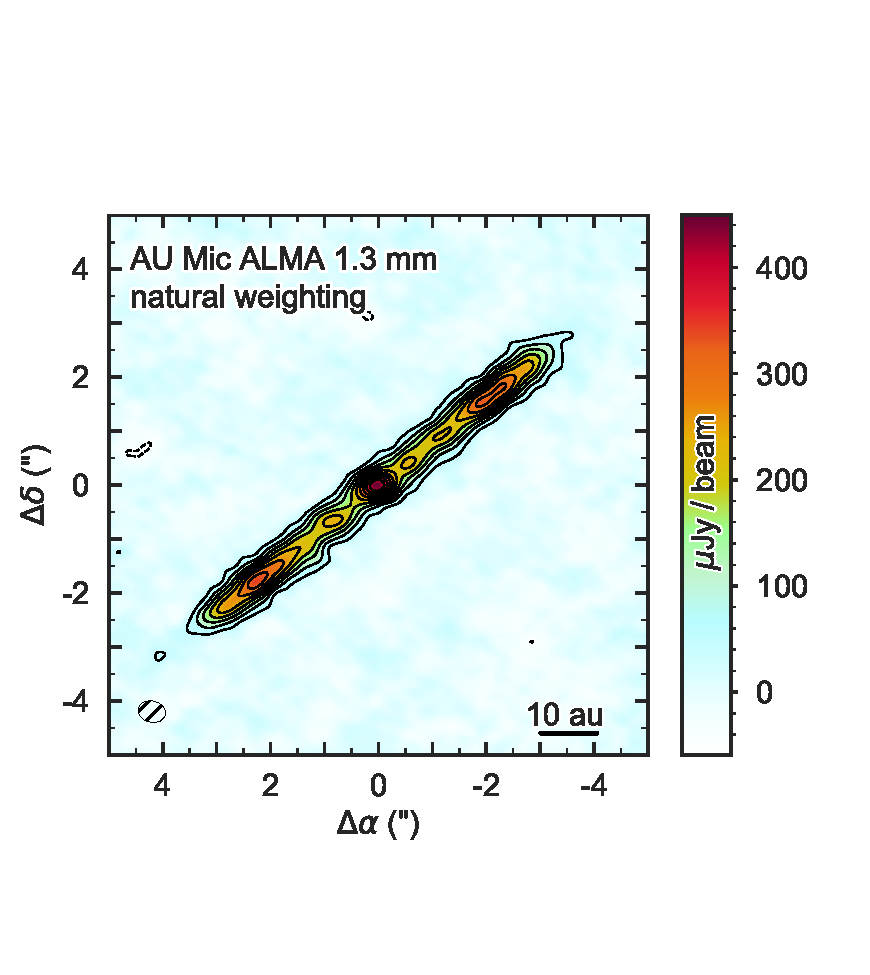
\includegraphics[width=\linewidth]{../figures/aumic_imaged}
  \caption{The AU Mic system imaged by ALMA at a wavelength of \SI{1.3}{mm}, using natural weighting with and without a Gaussian taper on the long baselines. 
  For the untapered weighting, the rms noise is \SI{15}{\mu Jy / beam} and the restoring beam has dimensions $\SI{0.52}{\arcsecond} \times \SI{0.39}{\arcsecond}$ with a PA of \ang[angle-symbol-over-decimal]{77.9}.
  The corresponding values for the tapered weighting are \SI{20}{\mu Jy / beam}, $\SI{0.87}{\arcsecond} \times \SI{0.71}{\arcsecond}$, and \ang[angle-symbol-over-decimal]{80.8}. 
  Contours are integer multiples of the three times the rms noise.
  The hatched ellipse in the bottom left of each pane designates the size and shape of the restoring beam.
  }
  \label{fig: aumic_imaged}
\end{figure}

Figure \ref{fig: aumic_imaged} shows the combined dust continuum emission from all three observations at \SI{1.3}{mm}; chromospheric emission from the M star is visible as a point source at the center of the image \citep{cranmer13}. 
The peak signal-to-noise ratio of dust emission is $\sim 23$.
Using the \texttt{MIRIAD} task \texttt{cgcurs}, we measure an integrated flux of \SI{4.97 \pm 0.08}{\milli Jy} enclosed within the $3\sigma$ contours of the naturally weighted image.  
Note that this value represents the combined emission from the disk \textit{and} the star. 
Faithfully disentangling the two components proved difficult, both because stellar and disk emission are blurred together in the central beam and because the stellar flux varied significantly across the three nights of observation (Table \ref{tab: params}).
Consequently, the most accurate way to isolate the disk flux from the stellar contribution is through parametric modeling (see \S \ref{section: analysis}) where the two components can be specified separately; our modeling yields a disk flux of \SI{4.80 \pm 0.17}{mJy}.
The ansa to the NW exhibits a maximum flux density of \SI{330 \pm 15}{\mu Jy/beam} at a separation of \SI{24.8 \pm 0.2}{au} and PA of $\ang[angle-symbol-over-decimal]{128.2} \pm 0.4$, while the ansa to the SE exhibits a maximum flux density of \SI{340 \pm 15}{\mu Jy} at a separation of \SI{29.0 \pm 0.2}{au} and PA of $\ang[angle-symbol-over-decimal]{128.7} \pm 0.4$. 
The peak flux densities of the ansae differ by less than the rms noise, indicating that there is no significant difference in brightness between the two limbs of the disk.
Indeed, the apparent flux asymmetry in these data is in the opposite direction of the apparent flux asymmetry in \cite{macgregor13}, providing further circumstantial evidence that there is no significant flux asymmetry at millimeter wavelengths. 
Additionally, the discrepancy in position angle between the two peaks falls within the estimated uncertainties and so we are not able to confirm the scattered light PA offset observed by \cite{boccaletti15}. 

\begin{figure}
  \centering
  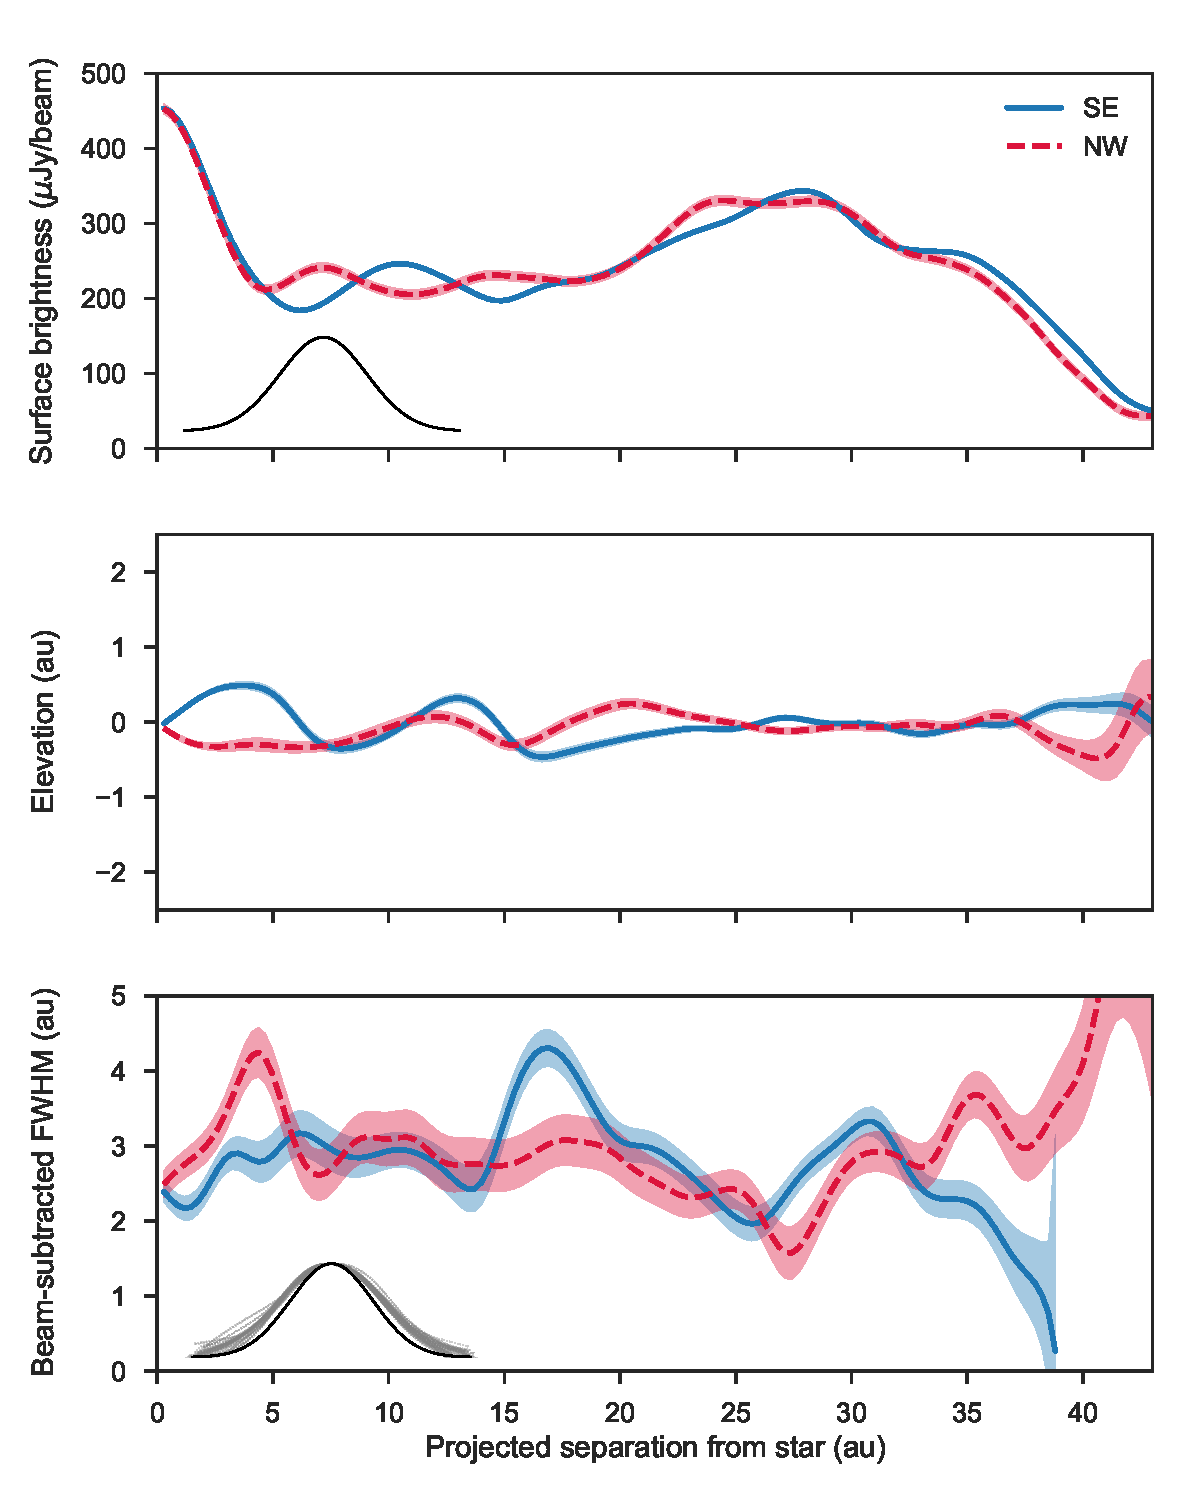
\includegraphics[width=.75\linewidth]{../figures/boccaletti_plots}
  \caption{
  Image-domain analysis of the AU Mic debris disk radial and vertical structure. 
  The solid blue line shows the southeast limb of the disk, while the dashed red line shows the northeast limb.
  From top to bottom, the three panes show i) the disk spine surface brightness with errors given by the rms noise, ii) the disk spine deviation from the midplane, and iii) the disk FWHM as a function of projected separation from the star. 
  The Gaussian traced by the dotted line in the first pane shows the projected width in the radial direction of the naturally weighted synthesized beam of the combined dataset.
%EIC: Following sentence ("The fact that ...") is not obvious to me just by looking at the figure.
%       In fact, the beam size as indicated by the Gaussian drawn on the top panel looks like it has a FWHM
%       of ~5 AU > the beam-subtracted FWHM plotted in the third panel. (I was pleased to see this
%       acknowledged in the main text, and to read about the various reasons why this is not necessarily
%       cause for alarm.)
%       I think the last sentence just needs to be reworded --- to acknowledge that the vertical beam
%       is technically larger than what is plotted, but that this is OK for various reasons discussed in
%       the main text under section 4.3. I gave it a stab.
%  The fact that the image-domain vertical height of the disk is in excess of the beam contribution implies that our data spatially resolve the vertical structure of the disk.
Although the last panel indicates a vertical disk FWHM that is technically smaller than the vertical FWHM of the beam,
it still represents a significant detection of vertical structure, for reasons explained in 
\S \ref{subsection: vertical analysis}.} 
  \label{fig: boccaletti}
\end{figure}

The vertical and radial structure of AU Mic's disk is traced in Figure \ref{fig: boccaletti}. 
At each radial location along the disk major axis, a one-dimensional Gaussian was fit to the vertical surface brightness profile.
The top, center, and bottom panes correspond respectively to the amplitude, centroid, and beam-subtracted FWHM of the Gaussian fits. 
Broadening effects of the synthesized beam in the vertical direction have been removed by subtracting in quadrature the Gaussian beam FWHM from the Gaussian fit FWHM.
In more physical terms, the three panes represent the intensity at the location of the disk ``spine,'' the spine's elevation from the midplane, and the disk FWHM.
We were unable to detect (in either the combined dataset or the three individual epochs) the intensity variations or excursions of the 
%EIC: added boccaletti18
disk spine from the midplane that characterize the fast-moving features observed by \cite{boccaletti15,boccaletti18}.
This is not entirely surprising, as both \cite{sezestre17} and \cite{chiang&fung17} suggest that the clouds are composed of sub-micron-sized grains which do not emit efficiently in the millimeter.

The disk is resolved across $\sim 17$ beams along the major axis, and cursory image-domain analysis indicates the disk is marginally resolved perpendicular to the major axis as well (Figure \ref{fig: boccaletti}, bottom pane).
$3\sigma$ emission as determined from the surface brightness profile in Figure \ref{fig: boccaletti} extends to a radial distance of $\sim \SI{43}{au}$ on the NW side and $\sim \SI{46}{au}$ on the SE side. 
We note the presence of local intensity maxima, nearly symmetric about the star at a distance of $\sim \SI{10}{au}$; it is unclear if these are real features of the disk or are artifacts of the rms noise or cleaning process. 
We examine the significance of these features in \S \ref{section: analysis}.

There is no evidence that the AU Mic system harbors a significant reservoir of molecular gas.
We set a $3 \sigma$ upper limit of \SI{0.07}{Jy.km.s^{-1}} on the CO~$\mathrm{J}=2-1$ integrated flux.
For a given excitation temperature, an upper limit on the total gas mass can be inferred from the upper limit on integrated flux.
We find the upper limit on the total gas mass to range between \SIrange[range-phrase=\ and\ ]{1.79e-7}{9.06e-7}{M_\earth} for excitation temperatures between \SIrange[range-phrase=\ and\ ]{10}{250}{K}.


\section{Analysis}
\label{section: analysis}
Previous studies of the scale height of debris disks have demonstrated a degeneracy between vertical structure, radial structure, and viewing geometry \citep[e.g.,][]{milli14}.  
In light of this, we adopt a modeling approach that combines appropriate ray tracing methods with a Markov Chain Monte Carlo (MCMC) algorithm in order to investigate the degree to which these known degeneracies impact our ability to measure the vertical structure of the disk.  

\subsection{Modeling Formalism}

We use the parametric structure and ray tracing disk code described in \cite{flaherty15}, itself an adaptation of earlier work by \cite{rosenfeld13}.
Synthetic sky-projected images are generated from a given temperature and density structure and are subsequently Fourier transformed to create model visibilities that can be directly compared to the interferometric data.

We assume the disk to be azimuthally symmetric and vertically isothermal. 
The disk vertical structure is set by the aspect ratio $h = H(r)/r$. 
At a given radius $r$, the vertical density profile is assumed to be Gaussian with a standard deviation equal to the scale height $H(r)$.
The dust opacity is set to \SI{2.3}{\cm^2.\gram^{-1}} \citep{beckwith90}, placing the model disk in the optically thin regime for the range of dust masses explored.
For an optically thin disk, the observed thermal emission is determined by both the surface density and temperature of the dust; to break the degeneracy between these two parameters, we assume that the dust grains are in blackbody equilibrium with the central star.
Thus the dust temperature at a distance $r$ from the host star is given by
\begin{align}
  T_{dust} (r) &= \left( \frac{L_{\star}}{16 \pi r^2 \sigma} \right)^{1/4}
\end{align}
where $L_{\star}$ is the bolometric luminosity of the star and $\sigma$ is the Stefan-Boltzmann constant. We assume that the radial surface density takes the form of a power law: 
\begin{align}
  \Sigma(r) &= 
  \begin{cases}
    \Sigma_c \, r^{p} \; \; \; \; & r_{in} \leq r \leq r_{out} \\
    0 \; \; \; \; &\mbox{otherwise} 
  \end{cases}
\end{align}
where $p$ is the power law exponent, and $r_{in}$ and $r_{out}$ are the disk inner and outer radius. 
$\Sigma_c$ normalizes the surface density structure for a given total dust mass $M_{dust}$:
\begin{align}
\Sigma_c &= \frac{M_{dust} \left(p + 2 \right)}{2 \pi \left[ r_{out}^{(p+2)} - r_{in}^{(p+2)} \right]}.
\end{align}

The observed disk PA and inclination $i$ are free parameters.
We adopt a stellar luminosity of \SI{0.09}{L_\sun} \citep{plavchan09} and a distance to the star of \SI{9.91 \pm 0.10}{pc}
%EIC: persnickety point / feel free to ignore: are you accounting for the change in stellar luminosity
%       that results from the new Gaia distance? It may not change 0.09 L_sun to the first significant figure,
%       so probably not worth worrying about. 
 \citep{vanleeuwen07};\footnote{We are currently re-running all models with the new Gaia distance of \SI{9.725 \pm 0.005}{pc}.} the observed \SI{1.3}{mm} stellar flux $F_\star$ is left as a free parameter for each observation date.
We note that the uncertainty in the stellar distance could affect the modeled disk mass and disk radial extent, while the 10\% systematic flux uncertainty could affect the modeled disk mass and stellar flux.
The spatial resolution of the resulting model sky image is set to \SI{0.3}{au} per pixel, chosen to be $\sim \SI{10}{\percent}$ of the spatial scale sampled by the longest baseline in the data. 
After the model image is generated by the ray tracing code, it is Fourier transformed into the visibility domain and sampled at the same spatial frequencies as the ALMA data with the \texttt{MIRIAD} task \texttt{uvmodel}.
This allows the model to be compared directly to the visibilities in the Fourier domain, where uncertainties are better characterized than in the image domain.
%EIC: spelling
A $\chi^2$ metric is used to
%asses
assess 
the quality of the fit.

We explore the parameter space of the model using the affine-invariant formulation of the MCMC algorithm described by \cite{goodmanweare10} and implemented in Python as \texttt{emcee} \citep{foreman-mackey13}.  
MCMC routines sample parameter space such that the density of samples in a given region is proportional to the local probability density, allowing estimation of the posterior probability functions themselves.
The process therefore not only identifies regions of high probability in parameter space, but also allows uncertainties and degeneracies between parameters to be determined from the correlations between the posteriors of each parameter. 
We assume uniform priors for all parameters; the dust mass was sampled in logarithmic space, formally equivalent to assuming a log uniform prior.
No prior bounds were placed on the logarithm of the dust mass.
Priors placed on the stellar flux and disk inner radius, width, and aspect ratio ensured that these parameters were always greater than zero, while the prior placed on the power law exponent ensured $-5 < p < 10$.
The position angle was confined to the range $\ang{1} < \text{PA} < \ang{360}$, and the inclination to $\ang{0} < i < \ang{90}$.
%EIC: "Leaving the inclination unbounded does not affect the preferred inclination ..."
%      This sounds funny and confusing for a couple reasons.
%      -- Leaving the inclination unbounded would seem to be the best possible thing
%      to do because "unbounded" implies "unbiased"; we don't want to affect the outcome in some unfair way.
%      -- Technically the inclination is bounded --- it is confined to be between 0 and 90 deg.
%      I think this needs to be reworded.
Leaving the inclination unbounded does not affect the preferred inclination; the MCMC chain simply converges to two positions symmetric about \ang{90}.
We performed several MCMC runs in order to investigate a variety of model formalisms. 
All runs used 50 walkers, and $10^5$ samples were drawn from each run to allow accurate statistical comparison between runs.


\begin{figure}
  \centering
  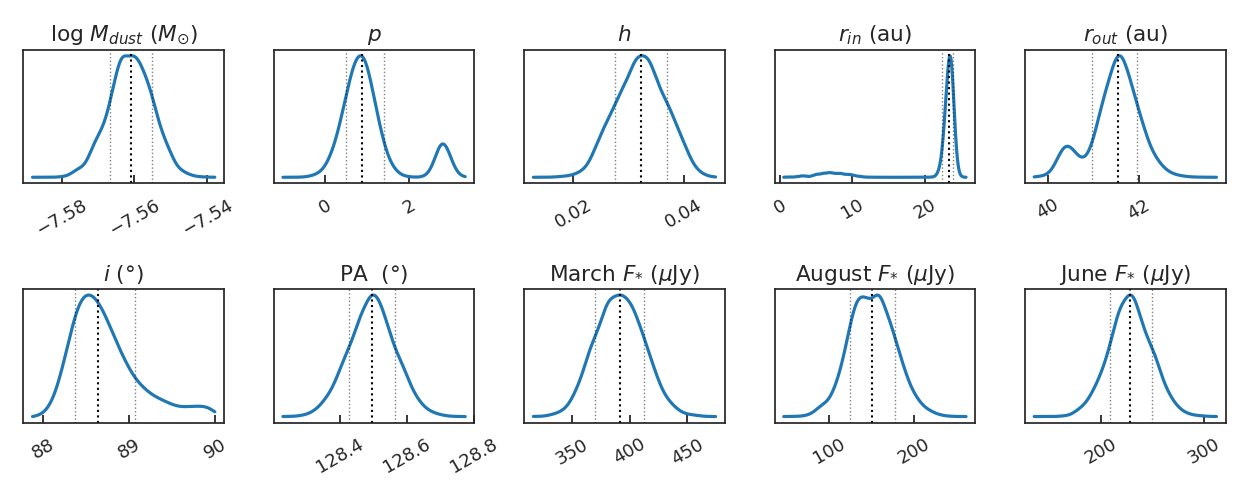
\includegraphics[width=\linewidth]{../figures/fiducial_kde}
  \caption{Kernel density estimates of the marginalized posterior probability distributions for the fiducial run. The central dashed line designates the median of each distribution while the outer lines mark the 16th and 84th percentiles ($1\sigma$ confidence intervals).}
  \label{fig: kde}
\end{figure}

Initially we varied ten parameters: the logarithm of the disk dust mass ($\log M_{dust}$), the disk inner radius ($r_{in}$), width ($\Delta r$), power law exponent ($p$), scale height aspect ratio ($h$), inclination ($i$), position angle (PA), and finally a separate stellar flux ($F_\star$) for each of the three observation dates. 
After the fact, the posterior distribution for $\Delta r$ was replaced by the outer radius posterior $r_{out} = r_{in} + \Delta r$ to allow for easier interpretation.
This model formalism resulted in a best-fit $\chi^2$ value of 626163.598 (reduced $\chi^2=2.053$), and we treat this parameterization as our fiducial model.

\begin{figure}
  \centering
%EIC: top left corner, single panel (BTW, I think most papers call these "panels", not "panes". But
%       if you want to keep calling them "panes", I don't mind; it reminds me of "window panes").
%       Is the y-axis really $h$? I don't think so. It should be some kind of probablilty density, right?
%       Same issue with the y-axis of every plot along the diagonal.
  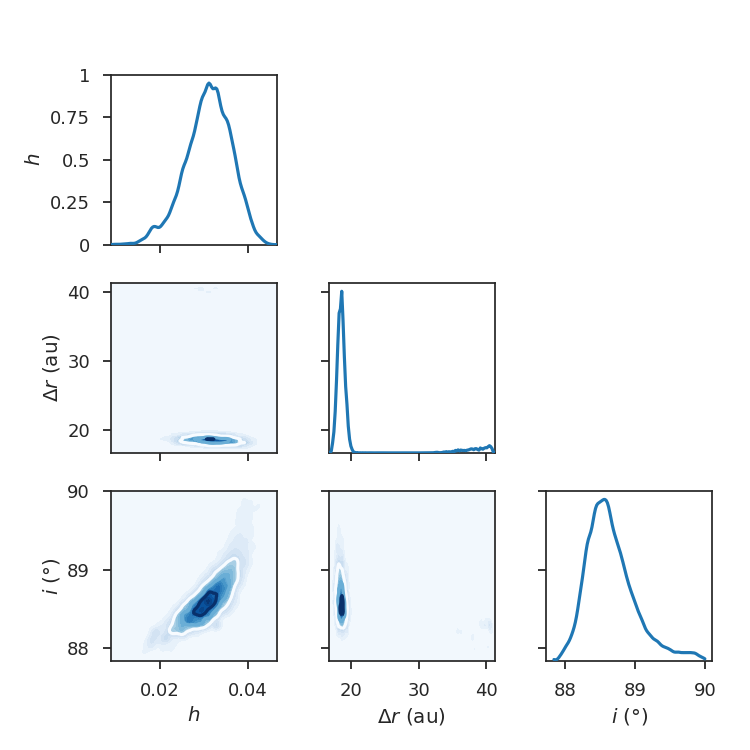
\includegraphics[width=0.9\linewidth]{../figures/degeneracy_corner}
  \caption{`Corner' plot showing degeneracies between a subset of the free parameters for the fiducial model.
  Two families of solutions are visible, and are most prominent in the $p$, $r_{in}$, and $r_{out}$ distributions.
  In addition, the two-dimensional slices through parameter space show limited degeneracies between radial structure, vertical structure, and viewing geometry.}
  \label{fig: degeneracies}
\end{figure}

\subsection{Investigating Radial Structure}
\label{subsection: radial analysis}

Marginalized posterior probability distributions for the fiducial model parameters are shown in Figure \ref{fig: kde}.
While the majority of the distributions are Gaussian, the three parameters that determine the radial structure of the disk ($p$, $r_{in}$, and $r_{out}$) exhibit slight bimodality. 
All three parameters are degenerate as can be seen from the `corner' plot in Figure \ref{fig: degeneracies}; in fact, the bimodality of the three parameters is a result of the existence of two distinct families of solutions in parameter space.
While the fiducial best-fit model has $p=0.8$, $r_{in}=\SI{24.0}{au}$, and $r_{out}=\SI{42.3}{au}$, a lower-likelihood family of solutions can clearly be seen in Figure \ref{fig: degeneracies}. The highest-likelihood model associated with this family has $p = 2.8$, $r_{in} = \SI{5.2}{au}$, and $r_{out} = \SI{41.0}{au}$.
More generally, mild degeneracies between the parameters determining vertical structure, radial  structure, and viewing geometry are visible, but the aspect ratio $h$ remains relatively uncorrelated with other aspects of AU Mic's structure.

The fiducial best-fit model image and residuals found in Figure \ref{fig: fiducial} provide further information as to the cause of the bimodal posterior distribution.
As can be seen from the residual map, the outer regions of the disk are reproduced well by the model; however $3\sigma$ residuals remain at the location of the star, as well as at symmetric positions at a separation of $\sim \SI{10}{au}$ on either side of the star. 
We note the symmetric residuals share the locations of the local intensity maxima described in \S \ref{section: results}. 
The convergence of these features leads us to consider the possibility of either a dust density enhancement (a ring) or reduction (a gap) in the inner regions of the disk. 
As a gap/ring would cause the radial surface brightness profile of the disk to deviate from that given by the simple power law used in our modeling, it could explain the bimodality in the posterior distributions of the parameters governing disk radial structure.

\begin{figure}
  \centering
  
  \subfloat[Fiducial run best-fit model and residuals.]{%
    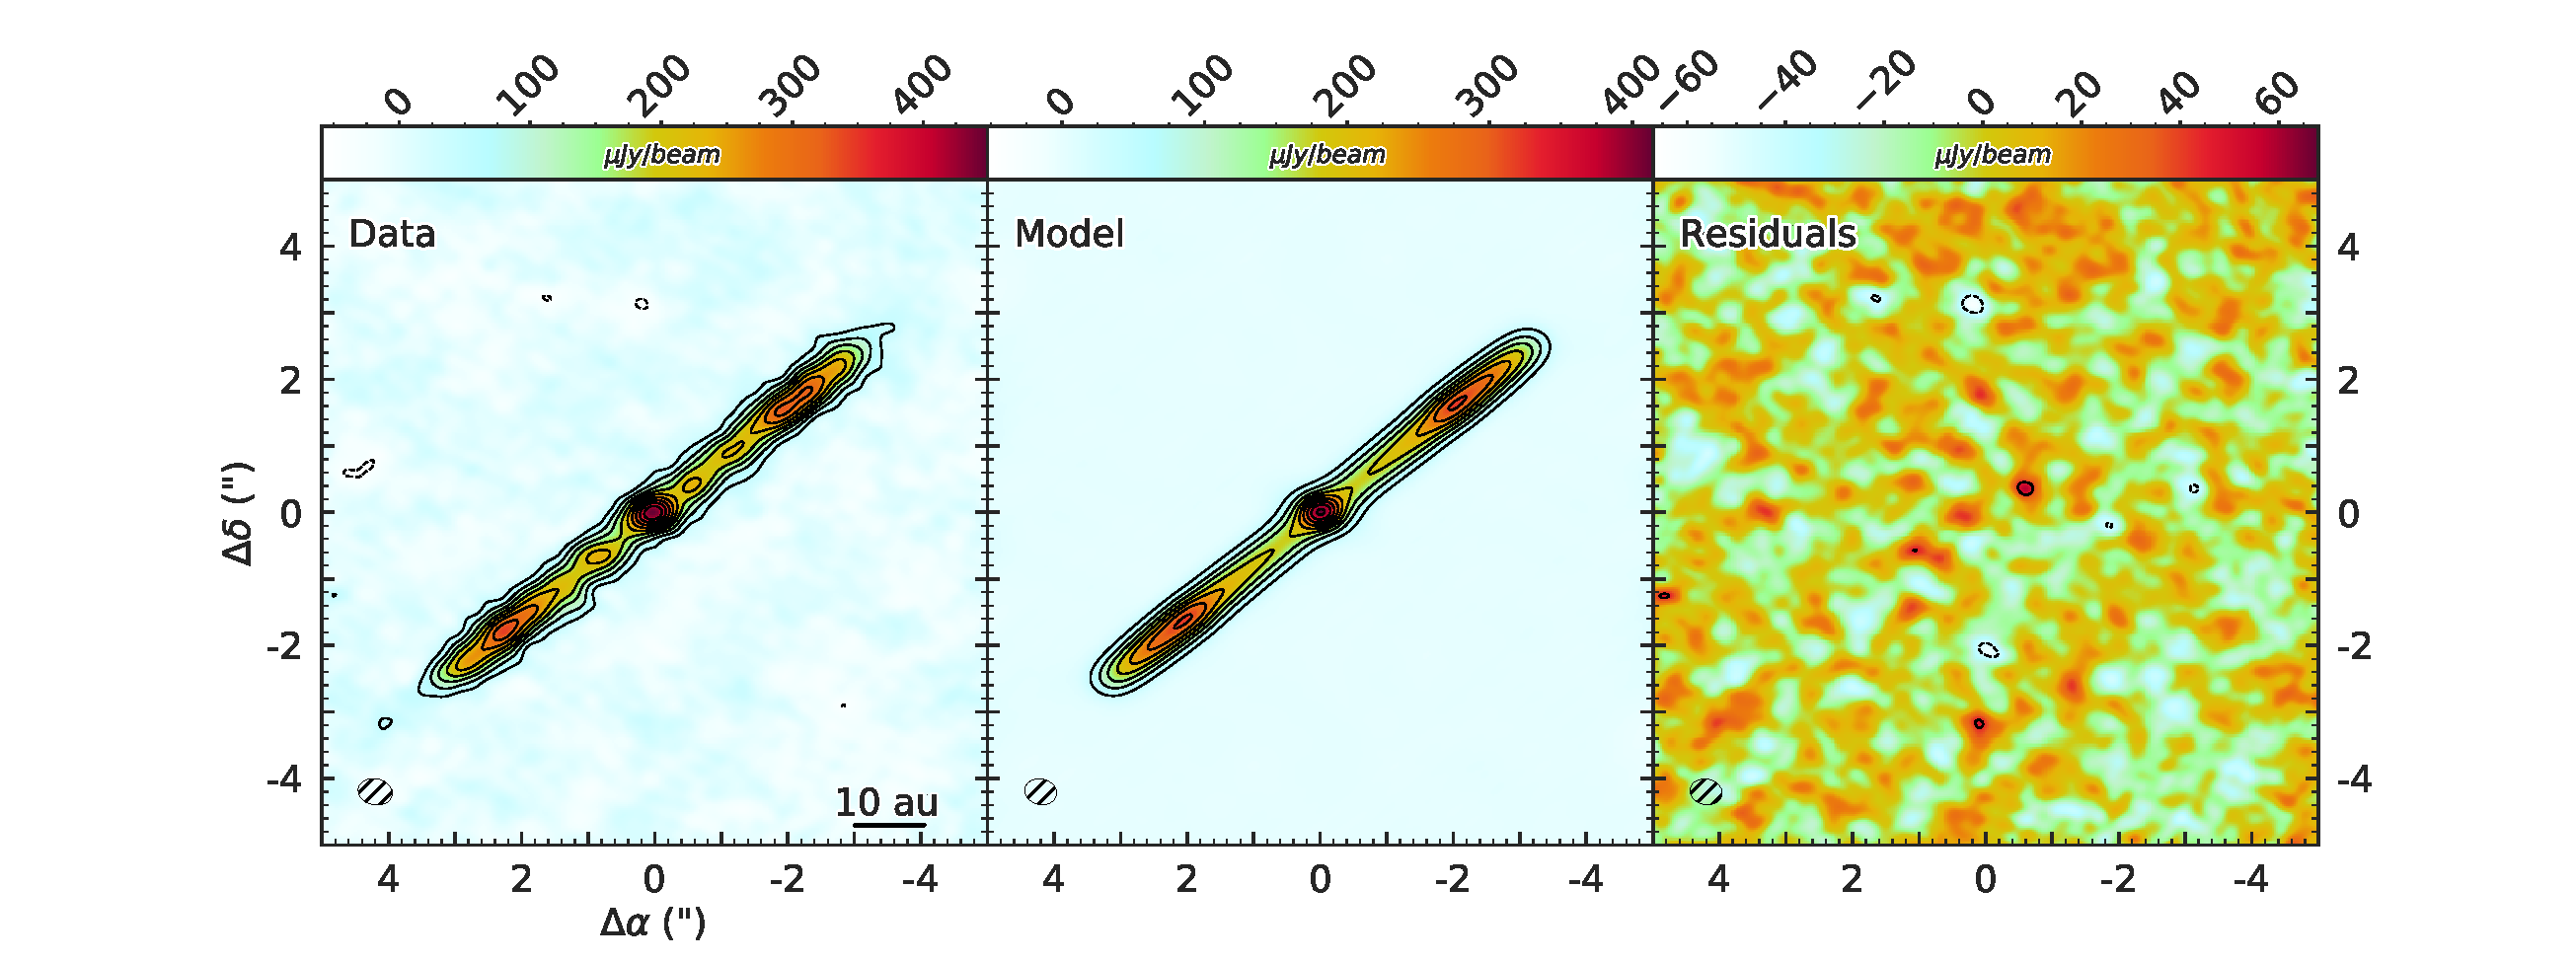
\includegraphics[width=0.77\linewidth]{../figures/fiducial_best_fit}%
    \label{fig: fiducial}%
    }\qquad
    
  \subfloat[Ring run best-fit model and residuals.]{%
    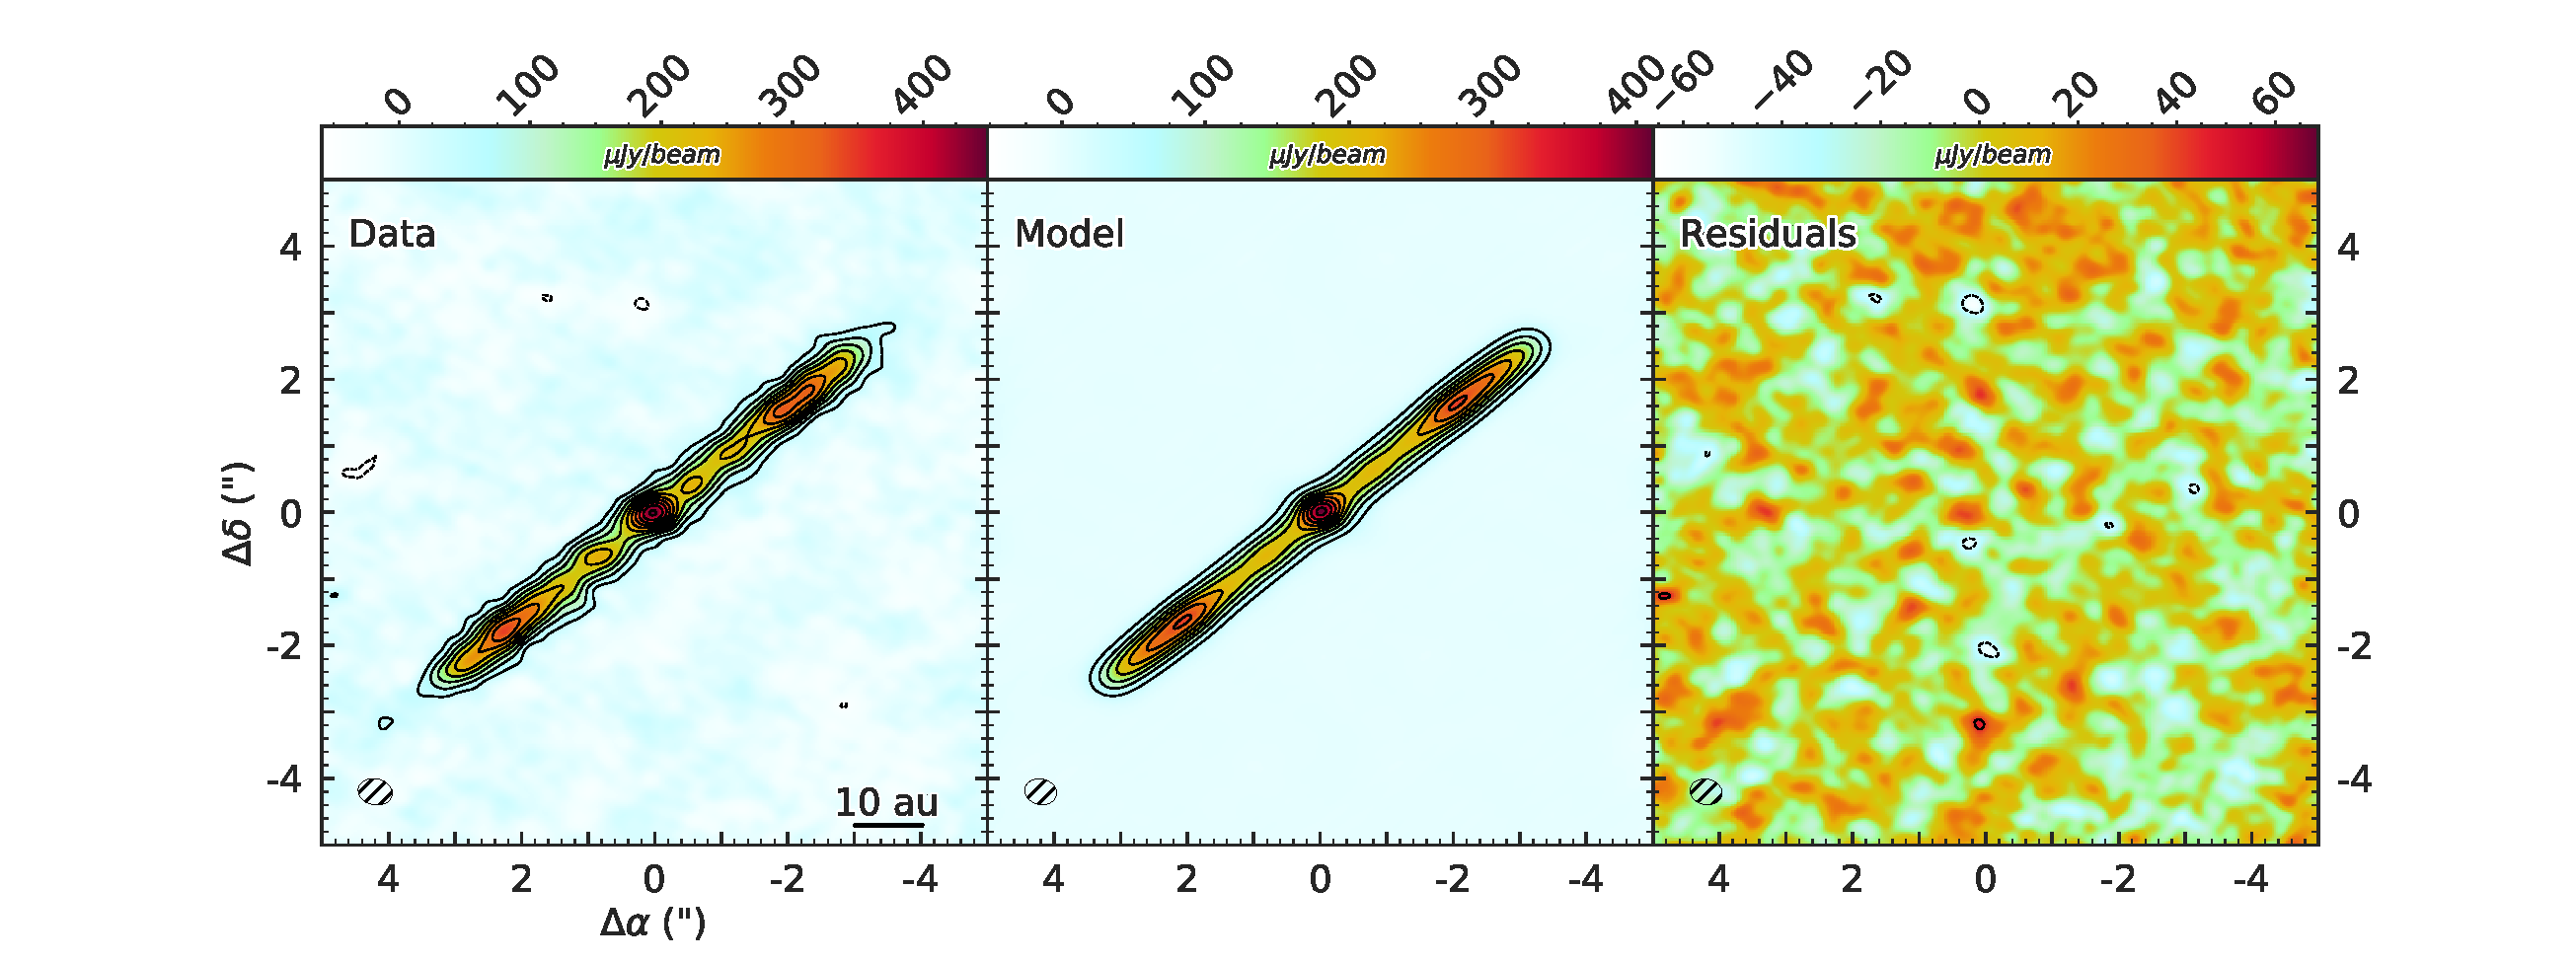
\includegraphics[width=0.77\linewidth]{../figures/annulus_best_fit}%
    \label{fig: ring}%
    }\qquad

  \subfloat['Skinny' disk run best-fit model and residuals.]{%
    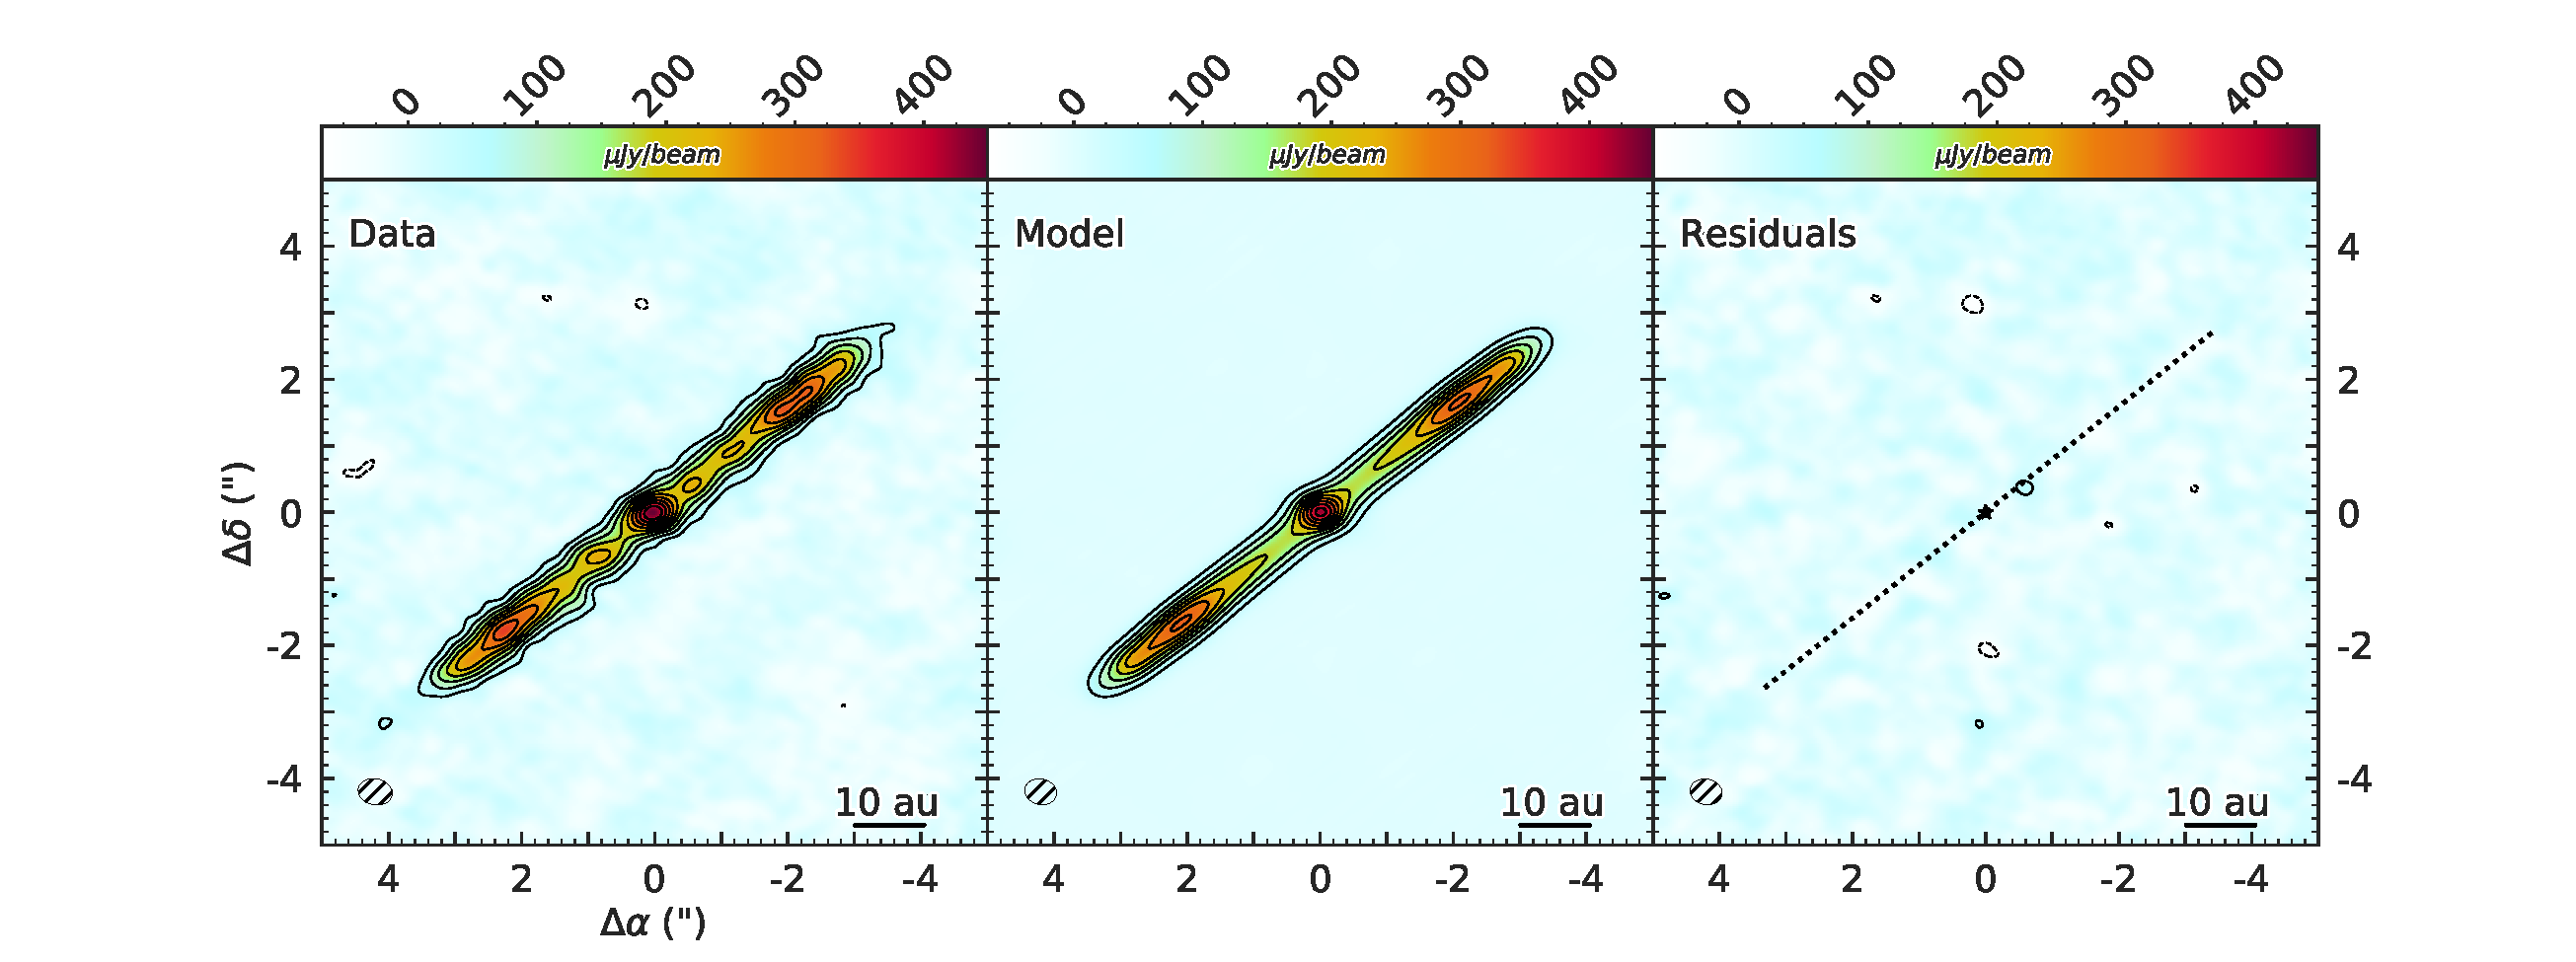
\includegraphics[width=0.77\linewidth]{../figures/skinny_best_fit}%
    \label{fig: skinny}%
    }\qquad
    
  \caption{Best-fit model image and residuals, sampled at the spatial frequencies of the ALMA data and cleaned using natural weighting. 
  Contours are integer multiples of the ALMA data $3\sigma$ confidence level. 
  For the fiducial model (a), $3\sigma$ residuals can clearly be seen at the location of the star and at symmetric positions $\sim \SI{10}{au}$ from the star. 
  Adding an additional ring of dust to the model (b) reduces these residuals by $\sim 25 \%$, but statistical analysis indicates that best-fit ring model does not conclusively describe the data better than the fiducial model.
  Fixing the scale height well below ALMA's resolution limits (c) results in a less statistically significant model, especially in the outer regions of the disk where ALMA is sensitive to the vertical structure of the disk.}
\end{figure}


We first explored the effects of adding a gap  to the inner regions of the disk. 
The gap inner and outer radii were left as free parameters and the dust density within the gap was set to zero.
The gap consistently converged to regions where the dust density was already zero (interior to the disk inner radius or exterior to the disk outer radius); we take this as evidence that the data are not well characterized by a gap.
As a next step, we experimented with adding a ring to the disk. 
The ring inner radius $r_{ring}$ was once again left as a free parameter and the ring width was fixed to \SI{0.3}{au}.
The ring was also characterized by a dust mass $M_{ring}$, which was evenly distributed across the radial extent of the ring. 
As can be seen in Figure \ref{fig: ring} this parameterization was better able to reproduce the `bump' in the radial surface brightness profile at $r \sim \SI{10}{au}$, reducing the best-fit model residuals by $\sim 25 \%$. 
However, $2 \sigma$ residuals are still present at the location of the bumps; the ring model's failure to accurately reproduce these features could be explained by the fact that the two local intensity maxima are not perfectly symmetric about the star. 
Image domain analysis indicates that the bump to the SE has a separation of $\sim \SI{11}{au}$, while the NW bump has a separation of $\sim \SI{8}{au}$  (Figure \ref{fig: boccaletti}). 
This discrepancy could be explained if the hypothetical ring were eccentric.

The median values and best-fit model parameters for the fiducial and ring parameterizations can be found in Table \ref{tab: params}. 
We use both the AICc, a form of the Aikake Information Criterion (AIC) corrected for finite datasets, and the Bayesian Information Criterion (BIC) to compare goodness of fit between models with different numbers of free parameters.  
The best-fit ring model is preferred to the fiducial model with $3.7 \sigma$ confidence on the AICc; conversely, the fiducial model is preferred to the ring model on the BIC with $\Delta \text{BIC} = 4.3$.
As such, we are not able to conclusively confirm the presence of an additional ring of mm dust grains in the AU Mic disk.

A model with a single $F_\star$ across all three dates was also investigated, but did not reproduce the data to the same degree of accuracy as the fiducial model.
Significant residuals were visible at the location of the star, and  a stellar flux varying by more than a factor of 2 over a period of months to years is preferred with $7.3 \sigma$ confidence by the AICc and with $\Delta \text{BIC} = 36.7$.

\begin{table}
  \centering
  \caption{MCMC Fitting Results}
  \label{tab: params}
  \renewcommand{\arraystretch}{1.2}
  \begin{tabular}{lrrrr}
  \toprule
    \multirow{2}{*}{Parameter} & \multicolumn{2}{c}{Fiducial} & \multicolumn{2}{c}{Disk + Ring} \\ 
    \cmidrule(lr){2-3} \cmidrule(lr){4-5} 
    & Median & Best Fit & Median & Best Fit \\
  \midrule
    $\log M$ (\si{M_\sun})   & $ -7.540 _{-0.006} ^{+0.006}$ & $-7.540$  & $-7.548  _{-0.007} ^{+0.007}$ & $-7.545$ \\
    $p$                        & $0.9     _{-0.4}   ^{+0.5}$   & $0.8$     & $0.8     _{-0.4}   ^{+0.6}$   & $0.9$     \\
    $h$                        & $0.031   _{-0.005} ^{+0.005}$ & $0.032$   & $0.027   _{-0.005} ^{+0.004}$ & $0.028$   \\
    $r_{in}$ (\si{au})         & $23.8    _{-0.9}   ^{ +0.6}$  & $24.0$    & $24.1    _{-0.9}   ^{+0.6}$   & $23.9$    \\
    $r_{out}$(\si{au})         & $42.3    _{-0.5}   ^{ +0.4}$  & $42.3$    & $42.3    _{-0.5}   ^{+0.4}$   & $42.4$    \\
    $i$ (\si{\degree})         & $88.6    _{-0.3}   ^{ +0.4}$  & $88.7$    & $88.27   _{-0.16}  ^{+0.22}$  & $88.3$    \\
    PA  (\si{\degree})         & $128.49  _{-0.07}  ^{+0.07}$  & $128.50$  & $128.50  _{-0.07}  ^{+0.07}$  & $128.48$  \\
    March $F_*$ (\si{\mu Jy})  & $390     _{-20}    ^{+20}$    & $390$     & $370     _{-20}    ^{+20}$    & $370$     \\
    August $F_*$ (\si{\mu Jy}) & $150     _{-30}    ^{+20}$    & $160$     & $150     _{-30}    ^{+20}$    & $140$     \\
    June $F_*$ (\si{\mu Jy})   & $220     _{-20}    ^{+20}$    & $220$     & $220     _{-20}    ^{+20}$    & $210$     \\
    $r_{ring}$ (\si{au})       &                               &           & $11.9    _{-1.8}   ^{+1.7}$   & $10.8$      \\
    $M_{ring}$ ($\si{M_\earth} \times 10^{-4})$  &             &           & $1.8     _{-0.7}   ^{+0.5}$   & $1.7$     \\
    $\ln$ Likelihood           & $-313087 _{-4}     ^{+2}$     & $-313082$ & $-313077 _{-5}     ^{+2}$     & $-313072$ \\
  \bottomrule
  \end{tabular}
\end{table}

\subsection{Investigating Vertical Structure}
\label{subsection: vertical analysis}

The posterior distribution for the aspect ratio $h$ suggests that the data are capable of measuring AU Mic's scale height despite the mild degeneracy between aspect ratio and other parameters like the radial structure and viewing geometry.  
Even when marginalized over these other parameters, the posterior distribution indicates a measured value of $h=\num{0.031 \pm 0.005}$, which translates to a $\sim 6 \sigma$ measurement of the scale height rather than an upper limit.
At the $\sim \SI{40}{au}$ outer edge of the disk, this aspect ratio implies a vertical scale height of \SI{1.2 \pm 0.2}{au}. 
The corresponding disk FWHM is \SI{2.8 \pm 0.5}{au}, consistent with an image-domain FWHM of $\sim \SI{3}{au}$ estimated from Figure \ref{fig: boccaletti}.
To verify that we in fact measured the scale height, we investigate a model parameterization in which the scale height is set to a value well below ALMA's resolution limits.
The aspect ratio is fixed at a value of $0.003$, so that even at the outer edge of the disk the scale height is $\sim \SI{3}{\percent}$ of the beam size along the disk's vertical axis.
If the disk is in fact resolved, such a `skinny' disk model should perform significantly worse than the fiducial model.
The best-fit model image and residuals are shown in Figure \ref{fig: skinny}.
The skinny model results in a significantly poorer fit to the data than the fiducial model with variable aspect ratio, with the best fits differing at the $3.9 \sigma$ level according to the AICc and by a value of 7.5 on the BIC.

The preferred disk FWHM is only $\sim 2/3$ the size of the combined-data beam projected onto the vertical axis of the disk.
While it may seem improbable that we measure a scale height below the image-domain spatial resolution of the combined data, our results can be explained by the following observations.
First, the beam size of the naturally weighted combined image ($\SI{0.52}{\arcsecond} \times \SI{0.39}{\arcsecond}$) is not wholly representative of the longest baselines in the data. 
The smallest naturally weighted beam FHWM from the three individual observations is \SI{0.30}{\arcsecond} (\SI{3}{au}; Table \ref{tab:observations}), while the spatial scale traced by the longest baseline is \SI{0.22}{\arcsecond} (\SI{2.2}{au}).
Second, the scale height $H$ refers to the disk height as measured from the midplane; the observable quantity that must be resolved in order to measure the scale height is actually the total vertical thickness $2H$.
Third, the scale height represents the standard deviation of a Gaussian distribution of dust particles that in fact reaches well beyond the extent of the scale height.
For example, considering that the peak SNR of the data is $\sim 23$ and that the vertical distribution of dust is assumed to be Gaussian, the SNR should remain above 3 over a total vertical extent of \SI{0.38}{\arcsecond} (\SI{3.8}{au}). 
The combination of these factors indicates that it is plausible that we are able to detect a scale height smaller than the resolution of the image-domain data.


\section{Discussion}
\label{section: discussion}

Parametric modeling suggests that AU Mic's debris disk is nearly edge on, exhibits an increasing surface density with radius until $\sim\SI{42}{au}$, and reaches a maximum scale height of $\sim\SI{1.2}{au}$.
There is also marginal evidence for an additional annulus of dust at $r \sim \SI{10}{au}$.
Here we compare the results of our analysis with previous studies of AU Mic's debris disk.

The geometric properties of the disk inferred from our modeling agree well with the literature. 
Our median inclination of $\ang[angle-symbol-over-decimal]{88.6}^{+0.4}_{-0.3}$ is consistent with previous estimates of the disk's inclination within uncertainties \citep{metchev05,krist05}.
The median PA of $\ang[angle-symbol-over-decimal]{128.49} \pm 0.07$ falls within uncertainties of measurements by \cite{macgregor13} and \cite{krist05}; however, the limb-averaged PA interior to \SI{50}{au} from \cite{metchev05} is $\ang[angle-symbol-over-decimal]{129.8} \pm 0.2$, and \cite{schneider14} report an optical-wavelength PA of $\ang[angle-symbol-over-decimal]{127.8} \pm 0.2$ between \SIrange{50}{100}{au}.
The preferred dust mass (\SI{0.01}{M_\earth}) is identical to the value derived from resolved \SI{1.3}{mm} imaging by \cite{macgregor13} and from low-resolution \SI{850}{\mu m} imaging by \cite{matthews15}; the latter quote a 20\% uncertainty.
Similarly, \cite{liu04} report \SI{0.011}{M_\earth} from unresolved \SI{850}{\mu m} observations.
\cite{strubbe&chiang06} calculate \SI{0.01}{M_\earth} by deriving a steady-state collisional cascade grain size distribution and fitting the disk's surface brightness and thermal spectrum to $V$- and $H$-band HST observations.
As discussed in \S \ref{section: results}, even a large gas excitation temperature of \SI{250}{K} implies a $3 \sigma$ upper limit on the total gas mass of only \SI{9.06e-7}{M_\earth}; combined with our preferred dust mass, this mass corresponds to an upper limit on the gas-to-dust ratio of $\sim 10^{-4}$.
Such a low dust-to-gas ratio excludes the possibility of gas influencing the millimeter grain kinematics, and thus our measurement of the scale height.

Our analysis indicates with high confidence that AU Mic exhibited long-term millimeter variability over the $\sim \SI{1.5}{yr}$ observation period. 
The stellar fluxes preferred by our modeling vary by more than a factor of two from one observation to the next, and are comparable to \cite{macgregor13}'s best-fit flux of \SI{320 \pm 60}{\mu Jy}.
It seems likely that this variability is distinct from the \SI{6}{minute} flare spanning two orders of magnitude that occurred during the June observations. 
That being said, we cannot rule out the possibility that the observations caught the star in varying states of flare decay, especially as \cite{white96} note that shorter-wavelength radio flares tend to have slower decay timescales.
Simulations of radio emission from low-mass stars allow for variability of more than a factor of two over the entire longitudinal extent of a star \citep{llama18}; it is also possible that different longitudinal regions of AU Mic were facing Earth during the three observations.
\cite{cox85} detect small-scale ($\sim 50\%$) variations over  a two-week period in \SIrange{2}{20}{cm} observations of AU Mic with the VLA, possibly due to `several independent mini-flares' or rotational modulation of the star.
In fact, factor of $\sim 2$ variability over months to years is typical of `quiescent' microwave emission from cool stars \citep{guedel94}.
Regardless of the origin of AU Mic's short- and long-term variability, we emphasize the importance of accounting for stellar emission/variability in observations of circumstellar disks around low-mass stars, especially in light of the Proxima Centauri flare discovered by \cite{macgregor18}.


\subsection{Radial Structure}
\label{subsection: radial discussion}

\begin{figure}
  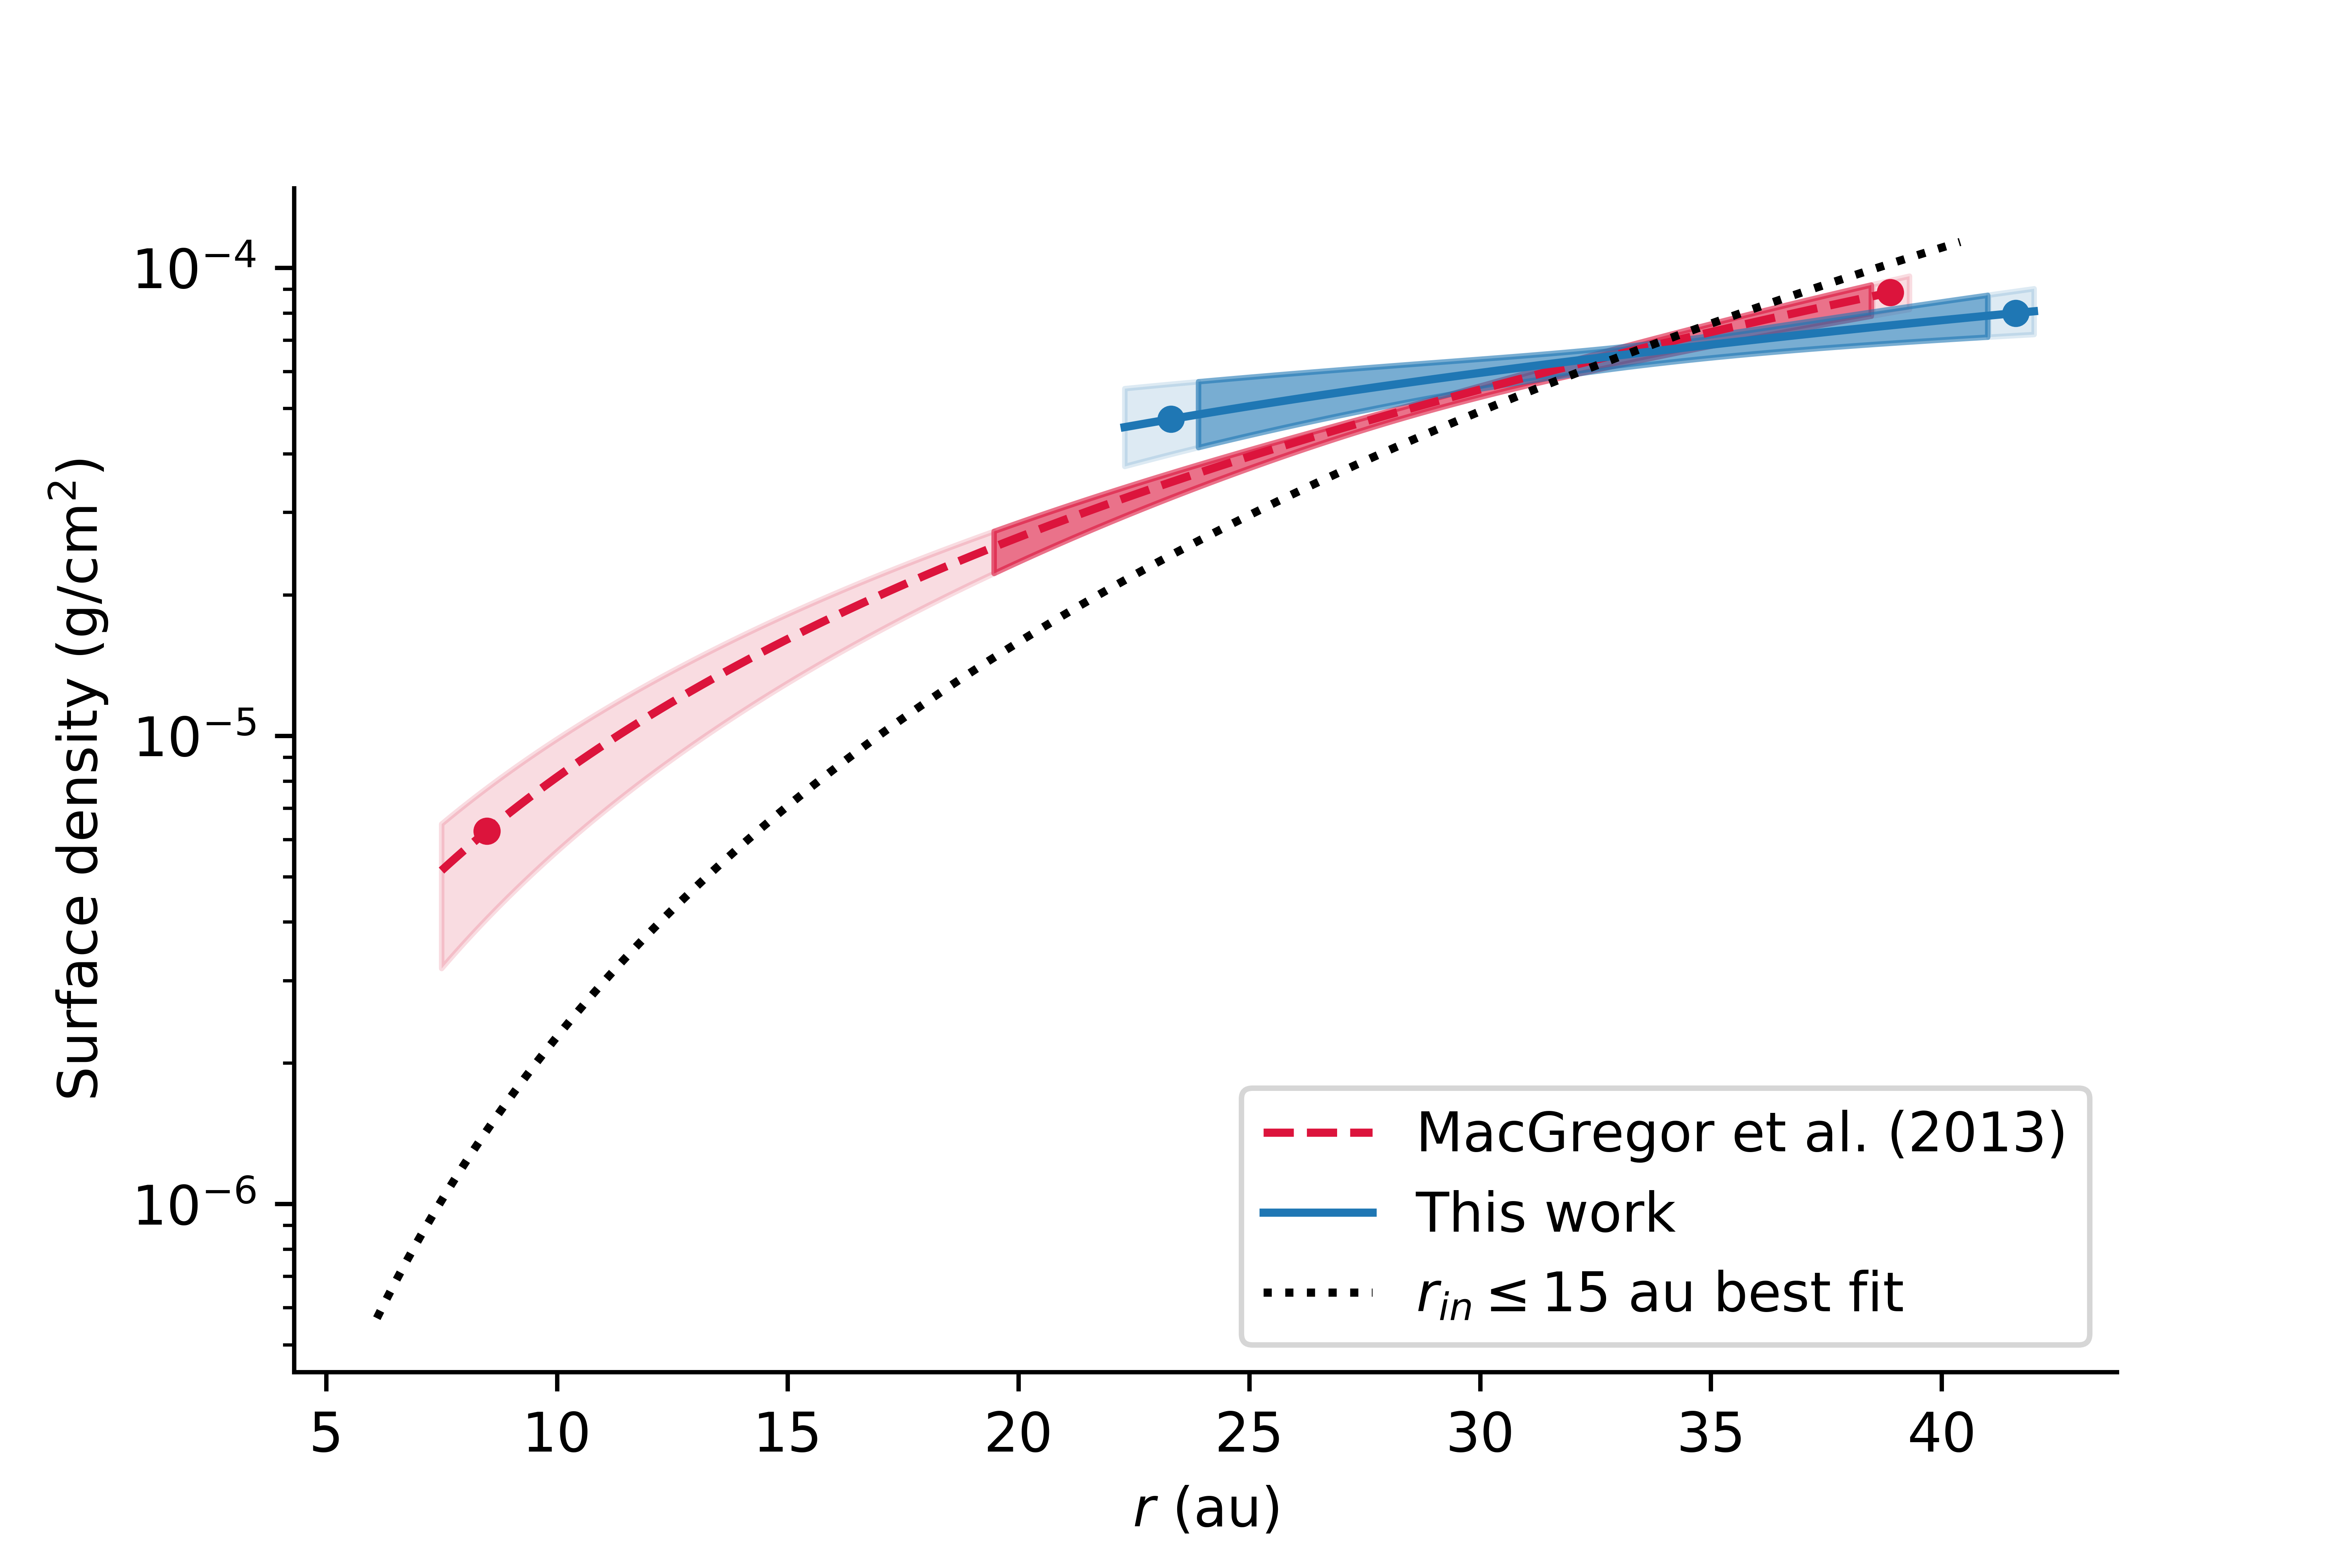
\includegraphics[width=\linewidth]{../figures/surface_density}
  \caption{
    Comparison between the best-fit surface density profiles obtained in \cite{macgregor13} (solid red line) and this work (dashed blue line).
    Also included is the best-fit surface density profile associated with the lower-likelihood family of solutions (dotted black line).
    The vertical extent of the shaded regions marks $1\sigma$ confidence intervals on the surface density. 
    The points designate the best-fit inner and outer radii for each model, and the horizontal extent of the more transparent shaded regions show $1 \sigma$ confidence intervals on the inner and outer radii.
    Not included in the uncertainties are the 10\% flux uncertainties of each observation.
    }
  \label{fig surface_density}
\end{figure}

Modeling of the radial structure discussed in \S \ref{subsection: radial analysis} is broadly consistent with the previous analysis of millimeter wavelength emission from the disk performed by \cite{macgregor13} as can be seen in Figure \ref{fig surface_density}. 
However, the factor of $\sim 2$ increase in spatial resolution introduces additional interpretive complexities when comparing the results.
%EIC
While our outer radius is only \SI{2}{au} larger than 
%than 
the previously reported value of \SI{40.3}{au} (confidence intervals are $\sim \SI{0.4}{au}$ for both measurements), things become more complicated when considering the inner radius $r_{in}$ and surface brightness power law index $p$.
In contrast to $r_{in} = 23.8_{-0.9}^{ +0.6}$ \si{au} preferred by our MCMC analysis, \cite{macgregor13} report $8.8_{-1.0} ^{+11.0}$ \si{au}.
Neither parameter is well constrained: the authors report a $3 \sigma$ upper limit of \SI{21}{au}, whereas conversely we find a $2 \sigma$ lower limit of $\sim \SI{1}{au}$.
Similar discrepancies arise in the posterior distribution for $p$, which is degenerate with $r_{in}$.
While \cite{macgregor13} finds $p=2.32_{-0.31}^{+0.21}$, we recover a median value of $p=0.9_{-0.4}^{+0.5}$.
In our analysis, the uncertainties in these two parameters arise from the existence of two families of solutions: one at $r_{in} \sim \SI{23}{au},\ r_{out} \sim \SI{42}{au},\ p \sim 0.8$ and another at $r_{in} \sim \SI{5}{au},\ r_{out} \sim \SI{41}{au},\ p \sim 2.8$ (Figure \ref{fig surface_density}).
The latter family, which has a lower likelihood, is probably associated with the local intensity maxima on either of the star examined in \S \ref{section: analysis}.
Our exploratory modeling of these features raises the possibility of an annulus of dust interior to the main disk---if such an annulus does exist, the $\sim 2$ times lower resolution observations from \cite{macgregor13} would probably not have been able to distinguish the annulus emission from that of the main disk.
In fact, an unresolved annulus would likely bias the inner radius preferred by the authors' modeling towards smaller values and could account for the differences in our characterization of the radial structure.

While the annulus model provides only a marginally significantly improved fit to the data, previous observations spanning a wide range of wavelengths have recovered surface brightness enhancements at the same projected stellocentric separation ($\sim~\SI{10}{au}$) as the hypothetical annulus.
A local maximum is present to the SE of the star at this separation in lower-resolution ALMA observations by \cite{macgregor13}, and there is a suggestive peak in the noise on the opposite side of the star as well.
Although these surface brightness enhancements do not attain $3 \sigma$ significance after subtraction of an axisymmetric model, the independent detection of these features in both data sets suggests that they may be real.  
\cite{schneider14} also observe an optical-wavelength `bump' $\sim \SI{13}{au}$ SE of the star and slightly elevated from the disk midplane (i.e. to the NE).
No matching surface brightness enhancement is observed on the NW side of the disk, which is obscured by the STIS occulting wedge for $r \lesssim \SI{12}{au}$.
On the other hand, the scattered light emission on the NW side is not symmetric about the midplane and the authors tentatively identify a warp below the midplane extending to a distance of $\sim \SI{45}{au}$ from the star.
They note that these features may share a common
%EIC
%causality, 
cause,
and posit that dust orbits in the inner disk are non-coplanar with those found at larger separations.

Near-infrared GPI obsevations presented in \cite{wang15} further corroborate the presence of a `bump' to the SE, characterized by a FWHM roughly triple the FWHM at an equivalent separation on the NW side of the disk. 
No features are detected at a corresponding separation to the NW.
Figure 4 of \cite{wang15} shows a composite map of the bump as seen by GPI, STIS, and ALMA; the common location of the bump in both scattered light and mm observations would indicate that the mm- and micron-sized grains are cospatial.
%EIC: It's a cascade. Everything is born from something bigger. That's why we call it the *birth* ring. 
%       SC06 covered the entire cascade, from the bottom of the cascade (micron) to 
%       the top (10 cm--1 meter; their equation 29), including the mm-wave SED (Figure 8). 
%       Actually, if anything, it's the larger cm-to-m-sized progenitors that are "mostly confined"
%       to the birth ring, since the micron-sized progeny are sent out onto eccentric orbits by 
%       stellar wind/radiation pressure. 
The micron-sized grains traced by scattered light,
%EIC: added
and all larger bodies ranging up to the cm-to-m sizes characterizing
the top of the collisional cascade,
are thought to 
%EIC: tweaked
%be mostly confined to 
originate from
a narrow `birth ring' at $\sim \SI{40}{au}$ \citep{strubbe&chiang06}. 
%EIC: I re-worded the last sentence.
%Thus, if the millimeter bump visible in both this work and in \cite{macgregor13} is indeed cospatial with the scattered light bump, it would suggest that the true stellocentric separation of the millimeter feature is $\sim \SI{40}{au}$ and that its apparent stellocentric separation of $\sim \SI{10}{au}$ is due to projection effects.
Thus it is possible that the millimeter bump visible in this work and in \cite{macgregor13}
are actually cospatial with the scattered light bump and that all features are located at a true
stellocentric separation of $\sim \SI{40}{au}$ (the apparent stellocentric separation
of $\sim \SI{10}{au}$ would be due to projection).

\subsection{Vertical Structure}
\label{subsection: vertical discussion}

As discussed in \S \ref{subsection: vertical analysis}, our MCMC analysis yields a median aspect ratio of $h~=~\num{0.031 \pm 0.005}$; at a reference point of \SI{40}{au}, this translates to a vertical scale height $H = \SI{1.2 \pm 0.2}{au}$.
This measurement is marginally consistent with values cited in the literature, ranging from roughly \SIrange{0.6}{2}{au} and derived from observations spanning the optical to the sub-millimeter.
\cite{schuppler17} place an upper limit of 0.05 on the \SI{1.3}{mm} opening angle (equivalent to the aspect ratio for small angles) by extracting the image-domain vertical profile from \cite{macgregor13}'s vertically unresolved ALMA observations, and estimate a visible-wavelength opening angle of 0.03 by reading off the vertical scale height from \cite{schneider14}'s STIS image of the disk.
\cite{metchev05} approximate a $H$-band Keck FWHM of $\sim \SI{4}{au}$ at a separation of \SI{40}{au};
\cite{krist05} fit a vertical Lorentzian profile to multicolor HST observations of the disk and find the FWHM interior to \SI{50}{au} to fall between \SIlist{2.5;3.5}{au}.

Because the measurements quoted above are determined from the observed vertical thickness of AU Mic's disk, they can be affected by the radial structure and viewing geometry of the disk as well as scattering effects. 
As such, parametric modeling provides a more reliable way to assess AU Mic's vertical structure.
\cite{krist05} report a FWHM between \SIlist{1.73;1.74}{au} at a separation of \SI{20}{au} from three-dimensional scattering models.
Collisional modeling can also be used to learn about AU Mic's vertical structure: collisional velocities---and thus dust production---are affected by the maximum eccentricity of planetesimal bodies $e_{max}$, which in turn can be related to the disk vertical stucture (see \S \ref{inferring mass} below). 
\cite{schuppler17} perform such modeling constrained by photometric observations spanning visible to millimeter wavelengths and quote a reference model opening angle of 0.015.
The authors go on to note that an opening angle of 0.005 better reproduces the disk spectral energy distribution (SED) in the long-wavelength regime beyond \SI{100}{\mu m}, but is unable to reproduce flux measurements for $\lambda \leq \SI{70}{\mu m}$.

In sum, estimates of AU Mic's vertical structure vary widely depending on the wavelength of observation, the techniques used, and the assumptions made.
Rigorous comparison between measurements in the literature is difficult---for example, \cite{krist05} assume a flared vertical profile while other authors use a linear parameterization for the scale height.
Nevertheless, some general statements may be made.
Values determined from optical and near-infrared observations range from roughly $H = \SI{1.2}{au}$ to \SI{2}{au} at a radius of \SI{40}{au}, while the values determined at least in part from mm observations range from $H = \SI{0.6}{au}$ to \SI{2}{au}, the latter being an upper limit. 
Estimates based on millimeter observations (including this work) tend to be smaller than those derived from shorter-wavelength observations, although the two wavelength regimes do not provide radically different values.

It is not unexpected that optical and infrared measurements of the scale height would exceed millimeter-wavelength estimates.
\cite{thebault09} suggests that the smaller grains traced by short-wavelength observations can be placed on inclined orbits by radiation pressure (and to first order, disk winds) even in the absence of large bodies dynamically stirring the disk. 
This effect preferentially excites smaller dust grains, `puffing' up the disk at mid-IR to visible wavelengths, while the larger grains that dominate emission at longer wavelengths remain near the midplane.
\cite{thebault09} proposes a `natural' minimum debris disk thickness of $h = \num{0.04 \pm 0.02}$ as seen at wavelengths smaller than \SI{50}{\mu \meter}.
The author also runs a collisional model tailored to the AU Mic system assuming no intrinsic dynamical excitation, and reports $H = \SI{1}{au}$ for $r \leq \SI{40}{au}$ when degraded to the resolution of scattered light images.
Although this scale height falls within the range of `natural' debris disk thicknesses, the 
%EIC: it's just a single author, right? Philippe Thebault? Or maybe this is an example of the "royal we"?
%authors stress 
author stresses
that this does not amount to an assertion that the disk is dynamically cold due to the simplicity of their model and fitting process.

In recent years, the vertical structure of several other debris disks has been tentatively resolved with ALMA.
$\sim \SI{5.5}{au}$ spatial resolution observations of 
CO~$\mathrm{J}=3-2$ and $2-1$ line emission from the edge-on $\beta$ Pic debris disk presented by \cite{matra17} suggest that the disk is resolved in the vertical direction.
The beam-subtracted apparent FWHM, determined in a similar manner as the bottom pane of Figure \ref{fig: boccaletti} in this work, ranges between $\sim$\SIrange[range-phrase=\ and\ ]{7}{12}{au} over the $\sim \SI{100}{au}$ radial extent of the disk.
Assuming an Keplerian rotation and edge-on inclination, the authors report the following scale height-radius relation:
\begin{align}
    H = 7.0 \pm 0.6 \times \qty(\frac{R}{\SI{85}{au}})^{0.75 \pm 0.02} \si{au}
\end{align}
where the scale height $H$ is the standard deviation of the Gaussian vertical density distribution.
For reference to this work, this corresponds to a scale height of \SI{4}{au} at a separation of \SI{40}{au}.
\cite{kennedy18} analyze $\SI{11.6}{au} \times \SI{13.1}{au}$ spatial resolution observations of the HR 4796A debris disk, reporting a marginal detection of the disk scale height.
The authors find that a vertically resolved ring (FWHM $= \SI{7 \pm 1}{au}$) is favored over a vertically unresolved ring
%EIC
%(FHWM 
(FWHM 
$< \SI{4}{au}$) with $\Delta BIC = 6.8$. 
This
%EIC 
%FHWM
FWHM
corresponds to a Gaussian standard deviation $H \approx \SI{3.0 \pm 0.4}{au}$ and, at the $\sim \SI{80}{au}$ radial location of the ring, a scale factor of $h \approx 0.038 \pm 0.005$.
Although the relative $BIC$ reported by the authors meets the condition for `strong' evidence of a statistically higher-quality fit ($\Delta BIC > 6$),
%EIC: "the fact that the ... nearly a factor of two smaller ... calls into question ..."
%       Seems an unfair criticism. Doesn't our work suffer from the same problem? 2/3 instead of 1/2,
%       as discussed in the last paragraph of our section 4.3?
%       Text needs to change here.
the fact that the preferred FWHM is nearly a factor of two smaller than the spatial resolution of the data calls into question the certainty of the measurement.
In sum, the vertical structure of debris disks is just beginning to be resolved in the millimeter thanks to the improvements in sensitivity and resolution provided by ALMA; to our knowledge, AU Mic exhibits the narrowest millimeter-wavelength scale height of any known debris disk.


\subsection{Inferring the Mass of Stirring Bodies}
\label{inferring mass}

Information regarding the bodies dynamically stirring AU Mic's disk can be recovered by relating the scale height to the dynamical excitation of the disk's dust grains.
As discussed by \cite{thebault09} and \cite{quillen07}, the planetesimals responsible for stirring the disk impart kinetic energy to the dust, perturbing them from a Keplerian orbit and thus increasing their eccentricity dispersion $\langle e^2 \rangle$. 
Here we define $\bar{e} = \sqrt{\langle e^2 \rangle}$ and $\bar{i} = \sqrt{\langle i^2 \rangle}$, where $\langle i^2 \rangle$ is the inclination dispersion of the dust grains.
In equilibrium there is an equipartition between the vertical and in-plane components of the velocities imparted to the grains, so $\bar{i} = {\bar{e}}/{2}$.
For low inclinations, inclination can be related to the observed aspect ratio using $\bar{i} = \sqrt{2}h$.
The interparticle relative velocity $\langle v_{rel} \rangle$ can then be determined directly from observables using the following relation \citep{wetherill&stewart93,wyatt&dent02}:
\begin{gather}
  \langle v_{rel} \rangle = v_{Kep}(r) \sqrt{\bar{i}^2 + 1.25 \bar{e}^2}
\end{gather}
where $v_{Kep}(r)$ is the Keplerian velocity at radius $r$. 
Adopting a stellar mass of \SI{0.5}{M_\sun} from the literature \citep{plavchan09,houdebine&doyle94} and taking $r = \SI{40}{au}$, $h=\num{0.031 \pm 0.005}$ yields $v_{rel} = \SI{360 \pm 60}{m/s}$.

The collisional velocities $v_{rel}$ of dust grains will never exceed the escape velocities $v_{esc}(a_{big})$ of the large bodies governing the disc's dynamics; $v_{rel} = v_{esc}(a_{big})$ only if velocity damping is not significant and all the bodies in the disk have had time to be gravitationally excited by the largest planetesimals. 
As such, we can use our estimate for $v_{rel}$ to place a lower limit on the escape velocity and thus size $a_{big}$ of bodies stirring the disk.
% \footnote{As pointed out by \cite{thebault09}, this is a rough approximation. $v_{rel}$ actually tells us about the product of the mass and surface densities of stirring bodies, $m_{big}\Sigma_{big}$ \citep{quillen07}.}
% This relationship allows us to estimate the mass $m_{big}$ and size $a_{big}$ of the bodies stirring the cascade.
Assuming a density of \SI{2}{\g.\cm^{-3}}, we find $a_{big} \sim \SI{340 \pm 60}{km}$ and $m_{big} \sim \SI{3.2 \pm 1.1e20}{kg}$, i.e. 2.5\% the mass of Pluto.
On the other hand, the disk may be in a steady state in which velocity damping is balanced with excitation (rather than damping being inefficient).
Under this condition the scale height provides an estimate of the total mass of stirring bodies, not their size.
To relate the observed disk scale height to the total mass of bodies stirring the disk, we refer to \cite{pan&schlichting12}'s theoretical models of steady state size-dependent velocity distributions in the collisional cascade.
Assuming a scale height of \SI{1.2}{au} at \SI{40}{au}, a stellar mass of \SI{0.5}{M_\sun}, and a dust mass of \SI{0.01}{M_\earth}, these models indicate a dynamical mass of $\sim\SI{1.5}{M_\earth}$.
If all of the \SI{1.5}{M_\earth} were locked up in a single body, it would have a radius of $\sim \SI{1.1}{R_\earth}$ assuming a mean density of \SI{5.5}{\g.\cm^{-3}} characteristic of Earth.

\begin{figure}
    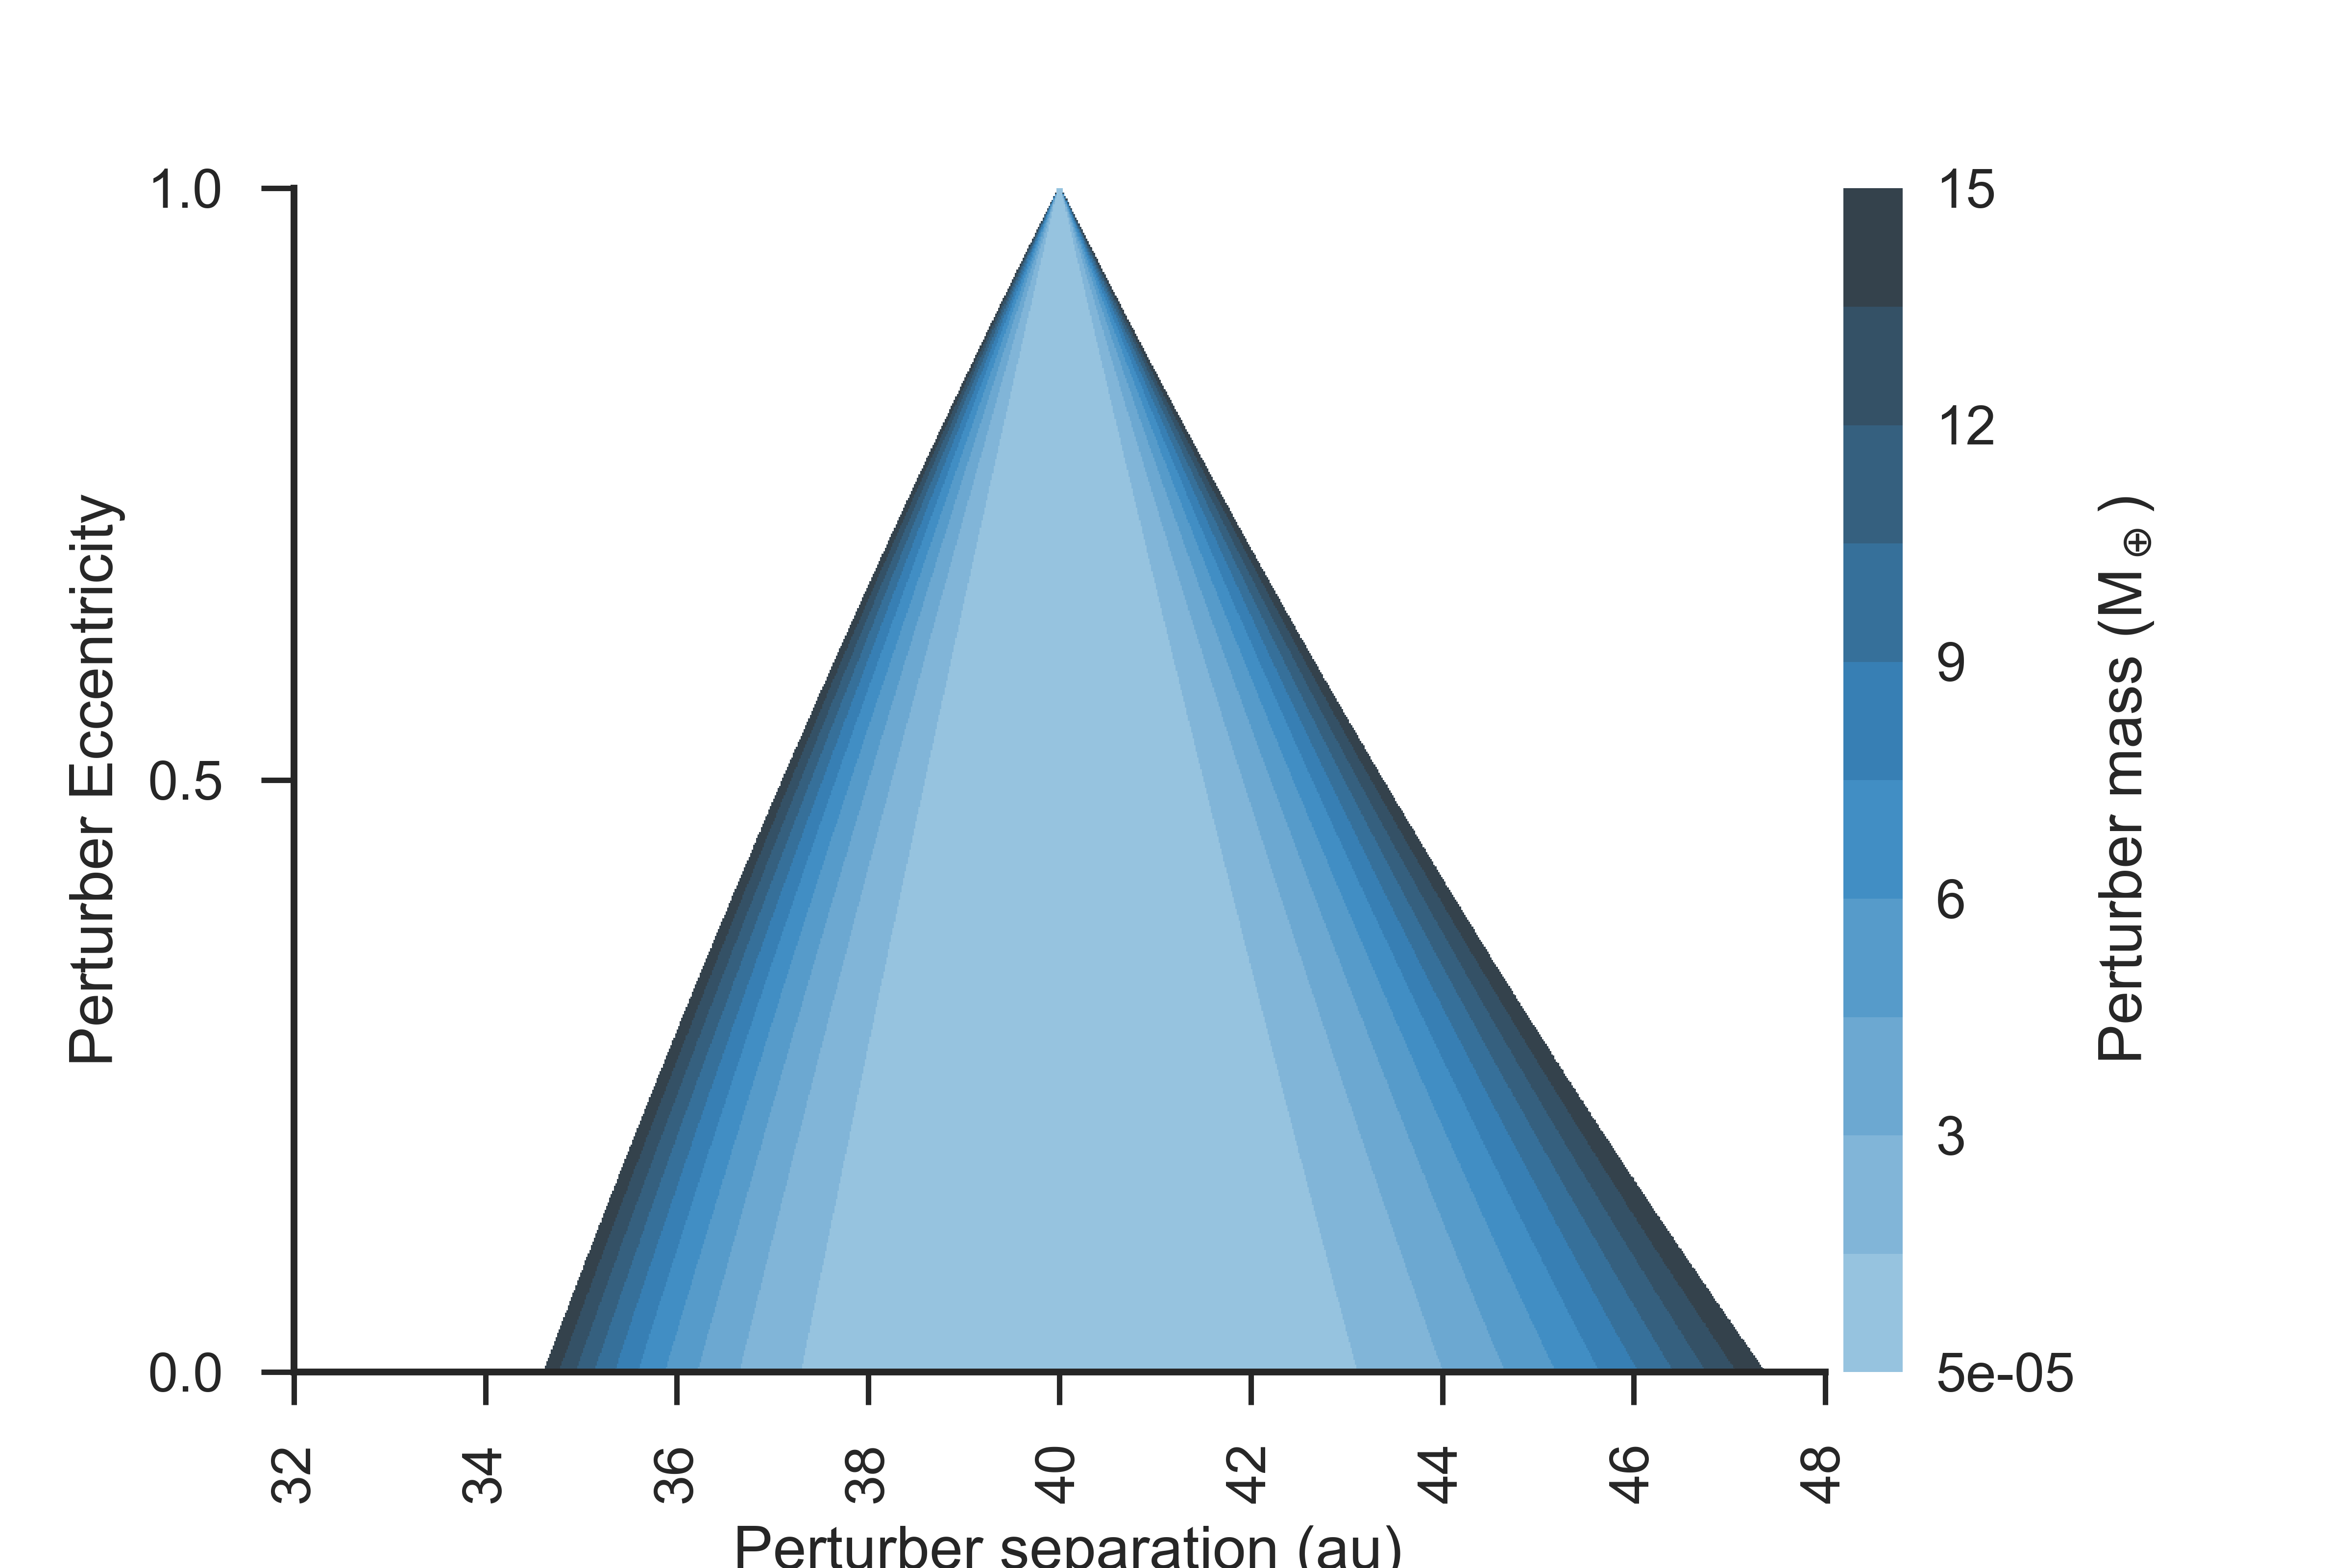
\includegraphics[width=\linewidth]{../../band6/plots/current/perturber_plot.png}
    \caption{An illustration of the relationship between the  mass, separation, and eccentricity of for a single stirring body. 
    The colormap shows the minimum stirring mass for a given orbital separation and eccentricity. 
    Colormap values range from \SI{5e-5}{M_\earth} (the lower limit placed on the perturber mass $m_{big}$) to \SI{15}{M_\earth} (slightly less than the mass of Neptune).
    The lightest shade of blue covers the entire range of perturber masses predicted by our calculations.}
    \label{fig: perturber}
\end{figure}

In sum, the largest bodies in the AU Mic disk cannot be smaller than \SI{340 \pm 60}{km} or they would not be able to stir the dust grains to the collisional velocities inferred from the measured scale height.
Conversely, the largest body stirring the disk cannot be larger than $\sim \SI{1.5}{M_\earth}$ or the scale height would exceed the value measured in this work.
It should also be noted that because the scale height measured at the outer edge of the disk is comparable to the spatial resolution of the data, and since scale height decreases with decreasing radius, the observations are only sensitive to the scale height near the $\sim \SI{40}{au}$ outer disk radius. 
If the disk is stirred by an ensemble of \SI{340}{km} planetesimals, they would necessarily be located within this outer region of the disk. 
%EIC: I agree with Hilke --- the $e$ dependence should be dropped (it refers to the Hill sphere radius at periapse,
%      and so is being used out of context here). Accordingly, Figure 7 should also be dropped, and this paragraph rewritten.
That being said, a planet is capable of stirring the disk at a distance of roughly five Hill Radii \citep{greenzweig&lissauer90}, defined as\footnote{To Margaret and Hilke: Meredith and I are a little confused here, as the expression for the Hill radius would imply that the stirring zone of a planet goes to 0 as its eccentricity goes to 1. Is this okay?}
\begin{align}
    r_{H} = a (1-e) \qty(\frac{m_p}{3M_\star})^{1/3}.
\end{align}
Thus if the mass were concentrated within a single \SI{1.5}{M_\earth} body, it could be located as far as \SI{3}{au} interior or exterior to the debris belt. 
Similarly, our measurement of the scale height excludes Uranus or Neptune analogs of mass $\sim \SI{15}{M_\earth}$ within \SI{6}{au} of the parent body belt. 
Figure \ref{fig: perturber} shows the relationship between the eccentricity, orbital separation, and mass of a single perturbing body.

%EIC: new last paragraph
The properties of the perturbers estimated in this work are consistent
with those inferred by \citet{chiang&fung17} on independent grounds
using the time-variable infrared observations by \citet{boccaletii15,boccaletti18}.
Our lower limit on the perturbing body size of $\sim$340 km fits with the
$\sim$400 km radius for their Varuna-like progenitor (for reference,
Varuna is among the larger objects in the Kuiper belt). Moreover, there should
be on the order of $10^3$ such objects according to their scenario (the argument
is as follows: since the lifetime of the debris left from the catastrophic disruption
of a Varuna-sized progenitor is $\sim$$3 \times 10^4$ yr \citep[][their equation 21]{chiang&fung17},
and since the age of the AU Mic system is $\sim$20 Myr, there must have been
20 Myr / $3 \times 10^4$ yr $\sim 700$ such progenitors over the system lifetime.
A population on the order of $10^3$ bodies
then yields an order-unity probability for observing the aftermath of a single
catastrophic collision today). An ensemble of $\sim$$10^3$ bodies each with a mass of
$4\pi/3 \cdot 2.5 \, {\rm g} \, {\rm cm}^{-3} \cdot (400 \, {\rm km})^3 \sim 10^{-4} M_\oplus$
amounts to a total mass of $\sim$$0.1 M_\oplus$, safely below the upper limit of $1.5 M_\oplus$
established by our present work.

\section{Conclusion}
\label{section: conclusion}

We have presented new \SI{1.3}{mm} ALMA observations of thermal dust emission from the debris disk around AU Mic at nearly double the angular resolution of previous observations. 
Both the vertical and radial structure of the disk are resolved.
MCMC analysis prefers an aspect ratio $h = 0.031$, corresponding to a vertical scale height $H = \SI{1.2}{au}$ in the outer regions of the disk.
Our analysis suggests that this is not a lower limit; a model with vertically resolved structure provides a statistically improved fit to the data over a model with unresolved vertical structure at a $4 \sigma$ confidence level.
Furthermore, the disk vertical FWHM derived from parametric modeling corresponds well with image-domain estimates of the beam-subtracted FWHM of the emission perpendicular to the disk plane.

By comparing our measurement of the scale height to the steady-state collisional modeling of \cite{pan&schlichting12} we are able to place constraints on the mass and size of bodies stirring AU Mic's disk.
In the lower-limit case where collisional velocity damping is inefficient, the stirring bodies would have a radius of \SI{340 \pm 60}{km}, corresponding to a characteristic mass $\sim 50$ times less than that of Pluto.
On the other hand, velocity damping may balance stirring; this condition allows us to place an upper limit of $\sim \SI{1.5}{M_\earth}$ on the mass of stirring bodies.
This is a dynamical mass, distinct from the lunar mass of dust grains inferred from the millimeter flux of the disk.
These results therefore rule out the presence of a gas giant or Neptune analog in the outer disk, but are suggestive of a significant 
%EIC: begin
population of large asteroids 
having a combined mass of less than one Earth. Such a population has been inferred on independent
grounds using time-variable infrared observations \citep{chiang&fung17}.
%or perhaps an Earth-mass planet stirring the dust distribution.  
%EIC: end

We see no indication of the fast-moving features detected by \cite{boccaletti15}, but the data are suggestive of an additional ring of dust at $\sim \SI{10}{au}$.
Models with a ring interior to the main disk provide a better fit to the data, but measures of statistical significance remain equivocal as to whether such models minimize the information lost in the modeling process.
Thus the presence of a ring remains uncertain. 
%EIC: begin
%EIC: maybe "obvious" to you, but not obvious to me. How is a ring at 10 AU "explained" by a planet?
%       I deleted the speculation, but left intact the reference to Peter Plavchan.
%If a secondary ring of dust does exist in the AU Mic debris disk, planets are of course an obvious explanation; 
P.~Plavchan et al.~(in preparation) propose a Jovian-mass exoplanet candidate interior to \SI{1}{au}, but AU Mic's stellar activity make it difficult to confirm the radial velocity detection.
%Even if the candidate is confirmed, it is unlikely that a planet so close to the star would be responsible for a ring at \SI{10}{au}.
%EIC: Sorry, I disagree strongly with the last sentence. Perhaps you can explain to me why a confirmed
%       detection of a planet (particularly one interior to 1 AU) would explain AU Mic's fast-moving features?
%       I am happy to discuss why I do not think such an explanation is viable, if you would like (skype/phone/email).
%That being said, a confirmed detection could provide a promising origin for AU Mic's fast-moving features.
%EIC: end

Looking forward, the scale height measurement presented in this work could be combined with other measurements of AU Mic's scale height at widely-separated (sub)millimeter wavelengths.
This would allow the size-dependent velocity dispersion and internal strengths of bodies in AU Mic's collisional cascade to be constrained, testing the assumption of collisional cascade theory that velocity dispersion is constant with grain size.
The ALMA Band 9 observations of AU Mic presented in the forthcoming work of
%EIC: begin
%Carter et. al 
Carter et al. 
(in preparation) may be able to provide such constraints.
Our measurements of the AU Mic system provide a proof of concept that spatially resolved observations of the vertical structure at millimeter wavelengths can constrain the presence of Uranus and Neptune analogs
%EIC: added
and even large Kuiper belt object analogues,
which are undetectable by
%other
standard 
planet-detection techniques.  
Applying this technique to other high-inclination debris disks with a range of central stellar masses will provide unique constraints on the prevalence of 
%Uranus and Neptune analogs 
large perturbing bodies
throughout the
%galaxy.
Galaxy.
%EIC: end

\section*{Acknowledgements}
C.D. is sponsored by a NASA CT Space Grant Undergraduate Research Fellowship and Wesleyan University's Research in the Sciences Fellowship.  
C.D., A.M.H., E.C., and K.F. gratefully acknowledge support from NSF grant AST-1412647.  
%EIC: I actually don't have a middle initial. But sometimes in papers I will use "I" to distinguish myself
%       from other E.C.'s. If Evan Carter has a middle initial, perhaps he can use his. If not, I am happy to use
%       my pen initial.
E.I.C. acknowledges support from the National Science Foundation.
This paper makes use of the following ALMA data:  ADS/JAO.ALMA\#2012.1.00198.S.  
ALMA is a partnership of ESO (representing its member states), NSF (USA) and NINS (Japan), together with NRC (Canada), MOST and ASIAA (Taiwan), and KASI (Republic of Korea), in cooperation with the Republic of Chile.  
The Joint ALMA Observatory is operated by ESO, AUI/NRAO and NAOJ.  
The National Radio Astronomy Observatory is a facility of the National Science Foundation operated under cooperative agreement by Associated Universities, Inc.

\software{
\texttt{CASA}  \citep{mcmullin07},
\texttt{MIRIAD} \citep{sault95},
\texttt{NumPy} \citep{van2011numpy}, 
\texttt{Astropy} \citep{astropy},  
\texttt{Pandas} \citep{mckinney}, 
\texttt{emcee} \citep{foreman-mackey13},
\texttt{Uncertainties}, \url{http://pythonhosted.org/uncertainties/} 
}
%===============================================================================
% APPENDIX
% \appendix 
%===============================================================================
% BIBLIOGRAPHY:
\clearpage
\bibliography{/Users/cdaley/Documents/Research/AU_Mic/writing/AU_Mic_bibliography.bib}
%===============================================================================
\end{document} 
